\documentclass[12pt,a4paper]{book}  %Вказівка класу документу
\usepackage[left=25mm,right=15mm,top=15mm,bottom=15mm]{geometry}  
\usepackage[T2A]{fontenc}
\usepackage[english, ukrainian]{babel}

\usepackage{indentfirst} %Відступи першого рядка абзацу
\usepackage{enumitem}  %Пакет для зручного переривання списку текстом

\usepackage[utf8x]{inputenc}
\usepackage{ucs}
\usepackage{amsmath}
\usepackage{amsthm}
\usepackage{amsfonts}
\usepackage{amssymb}

\usepackage{tikz}
\usepackage{verbatim}
\usepackage{setspace}

\author{Біляй Юрій Петрович}

\title{Лабораторний практикум з курсу \\ Програмування робототехнічних систем \\ спеціальність: Середня освіта (Інформатика)}

\onehalfspacing

%\ifx\pdfoutput\undefined
\usepackage{graphicx}
%\else
%\usepackage[pdftex]{graphicx}
%\fi

\input{CodeHighlights.tex}
\usepackage{color} %% это для отображения цвета в коде
\usepackage{listings} %% собственно, это и есть пакет listings

\usepackage{caption}
\DeclareCaptionFont{white}{\color{white}} %% это сделает текст заголовка белым
%% код ниже нарисует серую рамочку вокруг заголовка кода.
\DeclareCaptionFormat{listing}{\colorbox{gray}{\parbox{\textwidth}{#1#2#3}}}
\captionsetup[lstlisting]{format=listing,labelfont=white,textfont=white}

\begin{document}

\lstset{ %
numbers=left,               % где поставить нумерацию строк
numberstyle=\tiny
}

\newcommand{\code}{\texttt}

\maketitle

\tableofcontents 

\chapter{Основи елетричних схем}

\section{Основні закони електрики}

\subsection{Закон Ома}
Закон Ома -- головний закон електрики $I = \dfrac{U}{R}$

\subsection{Потужність}
Потужність -- міра швидкості зміни електричної енергії в іншу форму $P=I\cdot U$

Знаючи закон Ома, потужність можна обчилити $P=I^2\cdot R = \dfrac{U^2}{R}$

В процесі роботи частина енегрії трансформується в тепло. Через це гріються комп'ютери, телефони та інша техніка.
$P = P_W+P_D$, де $P$ -- споживча потужність, $P_W$ -- корисна потужність, $P_D$ -- потужність, що переходить в нагрівання.

\subsection{Коротке замикання}

З'єднання плюс і мінус напряму, за законом Ома, ожначає дуже велику силу струму і як наслідок до дуже великої потужності нагріванння, що у результаті спричиняє згоранння. Такий процес називається коротким замиканням. Ніколи не допускайте його появу, ні за яких обставин!

\subsection{Послідовне з'єднання}

При послідовному з'єднанні сила струму на кожному споживачеві однакова, а напруга падає в кожному наступному споживачеві.

\subsection{Паралельне з'єднання}

При паралельному з'єднанні напруга навколого кожного споживача однакова. Сила струму залежить від опору кожного окремого споживача.

\section{Основні компоненти}

\subsection{Конденсатор}

Конденсáтор (англ. capacitor) -- система з двох чи більше електродів (обкладок), які розділені діелектриком, товщина якого менша у порівнянні з розміром обкладок. Така система має взаємну електричну ємність і здатна зберігати електричний заряд.

Конденсатор є пасивним електронним компонентом і широко застосовується в електронних схемах для блокування постійного струму, пропускаючи змінний струм.

Конденсатор це маленький акумулятор який швидко заряджається і швидко розряджається.

\paragraph{Основні характеристики}


%\begin{table}
%\caption{Характрестики конденсаторів}
\begin{center}
\begin{tabular}{|l|c|c|}
\hline
\textit{Назва} & \textit{Позначення} & \textit{Одиниці виміру} \\
\hline
Ємність (номінал) & $C$ & Фарад \\
\hline
Точність (допуск) & $\pm$ & $ \% $ \\
\hline
Максимальна напруга & $V$ & Вольт \\
\hline
\end{tabular}
\end{center}
%\end{table}

\textit{Електролітичний конденсатор} має плюс і мінус, мінус відрізняється більш короткою ніжкою і/або білою смугою на корпусі.

\begin{figure}[h!]
\center{\includegraphics[height=1in]{images/ElectrolyticCapacitor.png}}
\label{ris:image}
\end{figure}

\begin{figure}[h!]
\begin{tikzpicture}[scale=.7]		
	\draw[line width=2] (0,1) -- (1,1);
	\draw[line width=2] (1.3,1) -- (2.3,1);		
	\draw[line width=2] (1.3,0) -- (1.3,2);
	\draw[line width=2] (0.77,0) arc (-30:30:2) ;
	\node[above left] at (2.1,-0.1) {$+$};
\end{tikzpicture}
\end{figure}




Керамічний конденсатор

\begin{figure}[h!]
\center{\includegraphics[height=1in]{images/CeramicCapacitor.png}}
\label{ris:image}
\end{figure}


\begin{center}
\begin{tikzpicture}[scale=.7]		
	\draw[line width=2] (0,1) -- (1,1);
	\draw[line width=2] (1.3,1) -- (2.3,1);		
	\draw[line width=2] (1.3,0) -- (1.3,2);
	\draw[line width=2] (1,0) -- (1,2);
\end{tikzpicture}
\end{center}

\subsection{Резистор}

Резистори належать до електричних компонентів, що застосовуються в схемах електротехніки та електроніки для обмеження сили струму та розподілу напруги. Резистори — найпоширеніші пасивні компоненти електронної апаратури, що використовуються як навантаження, споживачі та подільники в колах живлення, як елементи фільтрів, шунти, в колах формування імпульсів і т.д. 

\paragraph{Основні характеристики.}

%\begin{table}
%\caption{Характрестики конденсаторів}
\begin{center}
\begin{tabular}{|l|c|c|}
\hline
\textit{Назва} & \textit{Позначення} & \textit{Одиниці виміру} \\
\hline
Опір (номінал) & $R$ & Ом \\
\hline		
Точність (допуск) & $\pm$ & $ \% $ \\
\hline
Потужність & $P$ & Ватт \\
\hline
\end{tabular}
\end{center}
%\end{table}

\begin{figure}[h!]
\center{\includegraphics[width=1.5in]{images/Resistor.png}}
\label{ris:image}
\end{figure}

\begin{tikzpicture}[scale=2]		
	\draw[line width=2] (0,0) -- (0.3,0) -- (0.4,0.2) -- (0.5, -0.2) -- (.6, 0.2) -- (.7, -0.2) -- (.8, 0.2) -- (.9, -0.2) -- (1,0) -- (1.3, 0);
\end{tikzpicture}

\begin{tikzpicture}[scale=2]		
	\draw[line width=2] (0,0) -- (0.3,0) -- (0.3,0.15) -- (1, 0.15) -- (1, -0.15) -- (.3, -0.15) -- (.3, 0);
	\draw[line width=2] (1, 0) -- (1.3, 0);
\end{tikzpicture}

\paragraph{Кольорове кодування резисторів.}

Наносити номінал резистора на корпус числами~-- дорого і непрактично: вони виходять дуже дрібними. Тому номінал і допуск кодують кольоровими смужками.

При з'єднанні резисторів \textit{послідовно} їх еквівалентною схемою буде резистор з опором, рівним сумі опору окремих резисторів:

    $$R=R_{1}+R_{2}+\dots +R_{N}=\sum _{i=1}^{N}R_{i}$$
    
При \textit{паралельному} з'єднанні резисторів обернена величина еквівалентного опору (провідність) дорівнює сумі обернених величин усіх опорів (провідностей).

    $$ \frac{1}{R} = \frac{1}{R_{1}}+\frac{1}{R_{2}}+ \dots + \frac{1}{R_{N}}= \sum_{i=1}^{N}\frac{1}{R_{i}}$$

\subsection{Діод}

Діод~-- електронний прилад з двома електродами, що пропускає електричний струм лише в одному напрямі. 

\paragraph{Основні характеристики.}

%\begin{table}
%\caption{}
\begin{center}
\begin{tabular}{|l|c|c|}
\hline
\textit{Назва} & \textit{Позначення} & \textit{Одиниці виміру} \\
\hline
Падіння прямо напруги & $V_F$ & Вольт \\
\hline		
Максимальна обернена напруга яку може стримати & $V_{DC}$ & Вольт \\
\hline
Максимальний прямий потік & $I_F$ & Ампер \\
\hline
\end{tabular}
\end{center}
%\end{table}

\begin{tikzpicture}[scale=1.5]		
	\draw[line width=2] (0,0) -- (0.5,0);
	\draw[line width=2] (0.5,0.35) -- (0.5,-0.35) -- (1.2, 0) -- (.5,.35);
	\draw[line width=2] (1.2,0) -- (1.7,0);	
	\draw[line width=2] (1.2,.35) -- (1.2,-.35);	
	\node[] at (0.1,-0.25) {$+$};	
	\node[] at (1.6,-0.25) {$-$};	
\end{tikzpicture}

\subsection{Світлоіод}

Світлодіод~-- вид діода, який світиться, коли через нього проходить струм від анода(+) до катода(-). Ніжка анода довша за ножку катоду.

\begin{figure}[h!]
\center{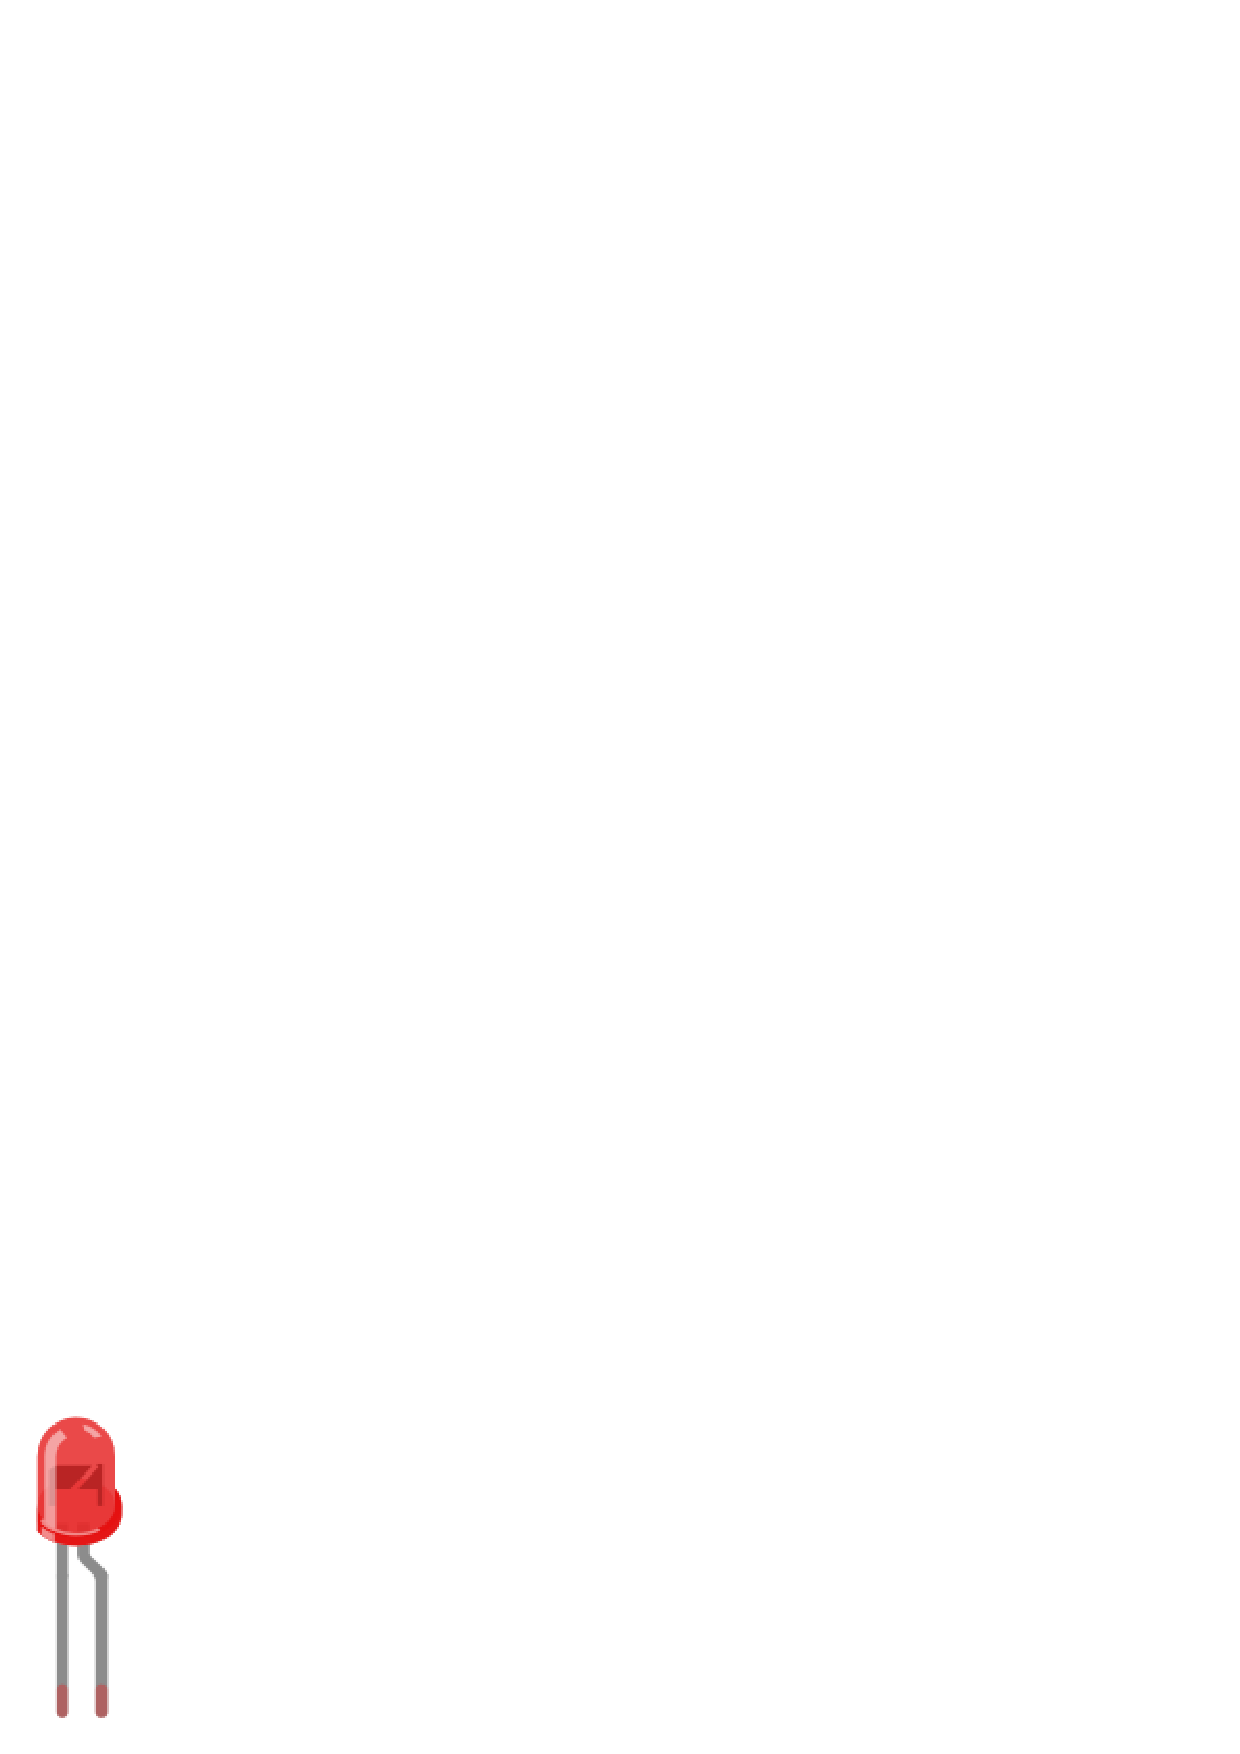
\includegraphics[height=1.2in]{images/LED.png}}
\label{ris:image}
\end{figure}

\begin{tikzpicture}[scale=1.5]		
	\draw[line width=2] (0,0) -- (0.5,0);
	\draw[line width=2] (0.5,0.35) -- (0.5,-0.35) -- (1.2, 0) -- (.5,.35);
	\draw[line width=2] (1.2,0) -- (1.7,0);	
	\draw[line width=2] (1.2,.35) -- (1.2,-.35);
	\draw[->, line width=2] (1.08, .36) -- (1.38, .66);	
	\draw[->, line width=2] (1.28, .25) -- (1.53, .50);	
	\node[] at (0.1,-0.25) {$+$};	
	\node[] at (1.6,-0.25) {$-$};	
\end{tikzpicture}


%\begin{table}
%\caption{}
\begin{center}
\begin{tabular}{|l|c|c|}
\hline
\textit{Назва} & \textit{Позначення} & \textit{Одиниці виміру} \\
\hline
Падіння прямої напруги & $V_F$ & Вольт \\
\hline		
Номінальни струм & $I$ & Ампер \\
\hline
Інтенсивність (яскравість) & $I_V$ & Кандела \\
\hline
\end{tabular}
\end{center}

Власний опір світлодіода після насичення досить малий тому без резистора, що обмежує струм, він перегорить.

\paragraph{Вибір потрібного резистора.}

Розрахуємо який резитор опору $R$ потрібно взяти щоб отримати оптимальний результат. Для прикладу нехай характеристики світлодіода який потрібно під'єднати такі: $V_F = 2.3\text{В}, I = 20\text{мА}$, напруга джерела живлення $V_{CC} = 5\text{В}$.

Знайдемо оптимальний опір $R$ і мінімально допустиму потужність резистора $P_R$.
Спочатку обчислимо яку напругу повинен взяти на себе резистор:
$U_R = V_{CC} - V_F = 5 \text{В} - 2.3\text{В} = 2.7\text{В}$.
За законом Ома знайдемо значення опору, за якого буде забезпечено таке падіння:
$R = \dfrac{U_R}{I} = \dfrac{2.7 \text{В}}{0.02 \text{А}} = 135 \text{Ом}$.
Таким чином при опорі більше за $135\text{Ом}$ яскравість буде нижчою за заявлену у специфікації виробу, при опорі меншому за $135\text{Ом}$ строк роботи світлодіода буде меншим.

Тепер знайдемо потужність, яку за такого процесу, резистору доведеться розсіювати:

$P_R = I^2 \cdot R = 0.02 \text{А}^2 \cdot 135 \text{Ом} = 0.054 \text{Вт}$.

Це означає, що за потужності резистора меншій за $54$ мВт резистор перегорить.

%\end{table}

\subsection{Кнопка}
Тактова кнопка~-- простий механізм, за допомого якого можна замкнтуи електричне коло поки кнопка натиснута.

\begin{figure}[h!]
\center{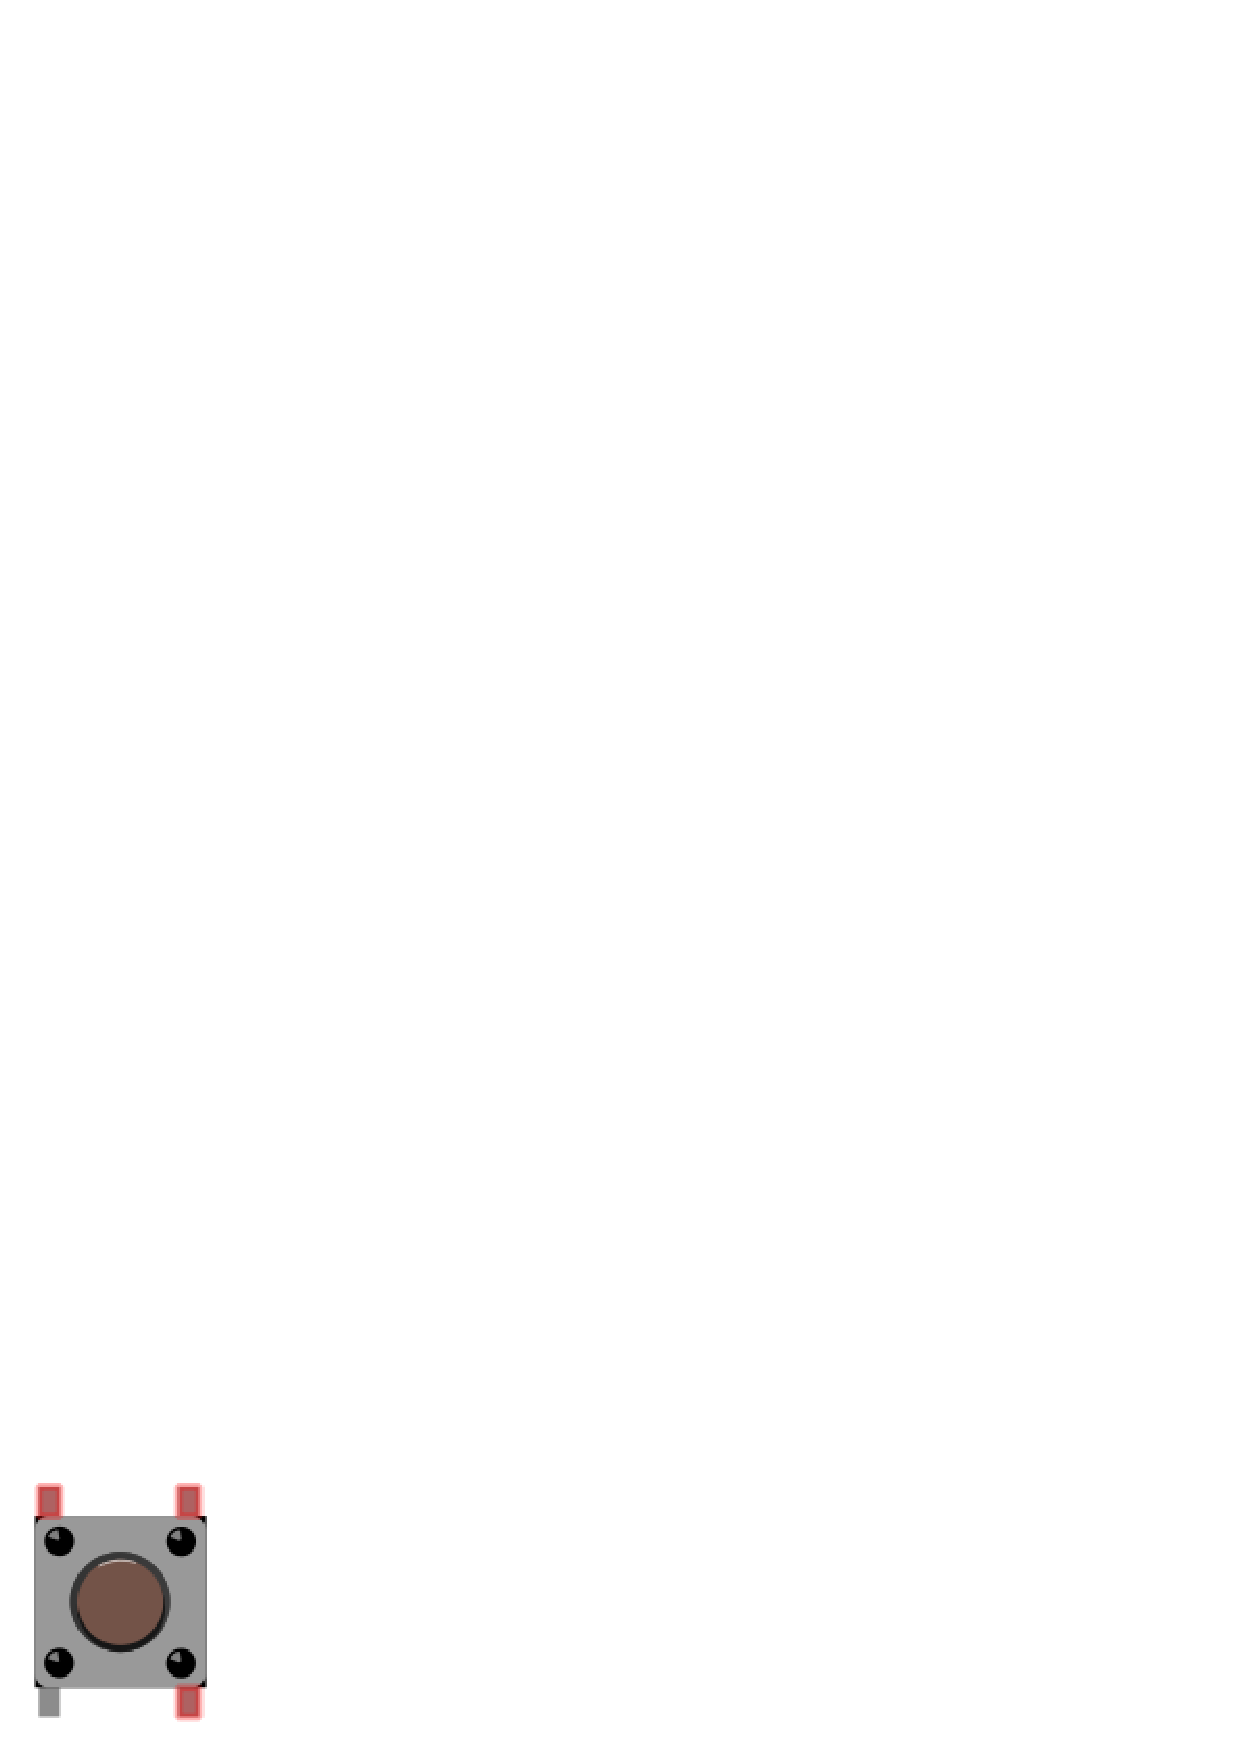
\includegraphics[height=1in]{images/Button.png}}
\label{ris:image}
\end{figure}

Кнопки з 4 контактами можна розглядати як 2 пари рельс, що з'єднуються під час натиснення.

\begin{tikzpicture}[scale=1.5]		
	\draw[line width=2] (0,0.5) -- (0.5,0.5) -- (0.5, -0.5) -- (0, -0.5);
	\draw[line width=2] (0.5,0) -- (0.7,0) -- (1.5, 0.3);
	\draw[line width=2] (1.5,0) -- (1.7,0);
	\draw[line width=2] (2.2, 0.5) -- (1.7, 0.5) -- (1.7, -0.5) -- (2.2, -0.5);	
\end{tikzpicture}

\begin{tikzpicture}[scale=1.5]		
	\draw[line width=2] (0,0) -- (0.7,0) -- (1.4, 0.4);
	\draw[line width=2] (1.4,0) -- (2.1,0);
	\draw [black, fill=black] (0.7,0) circle [radius=0.07];
	\draw [black, fill=black] (1.4,0) circle [radius=0.07];
\end{tikzpicture}	

Під час замикання та розмикання контактів кнопки між пласниами кнопки виникають мікроіскри, за рахонок чого відбуваються десятки перемикань за декілька мілісекунд. Це явице називається "дрижанням" (англ. \textit{bounce}). Цей ефект потрібно враховувати якщо потрібно фіксувати натиснення.

Поки кнопка натиснута, вихідна напруга $V_{out} = V_{cc}$, але коли вона відпущена, $V_{out} \neq 0$. Кнопка і провідники в цьому випадку працюють як антена, і $V_{out}$ буде «шуміти», приймаючи випадкові значення «з повітря».

Поки з'єднання немає, необхідно створити резервний шлях для визначення напруги. Для цього використовують один з двох варіантів.

\begin{figure}[h!]
\caption{Схема з стягуючим резистором}
\center{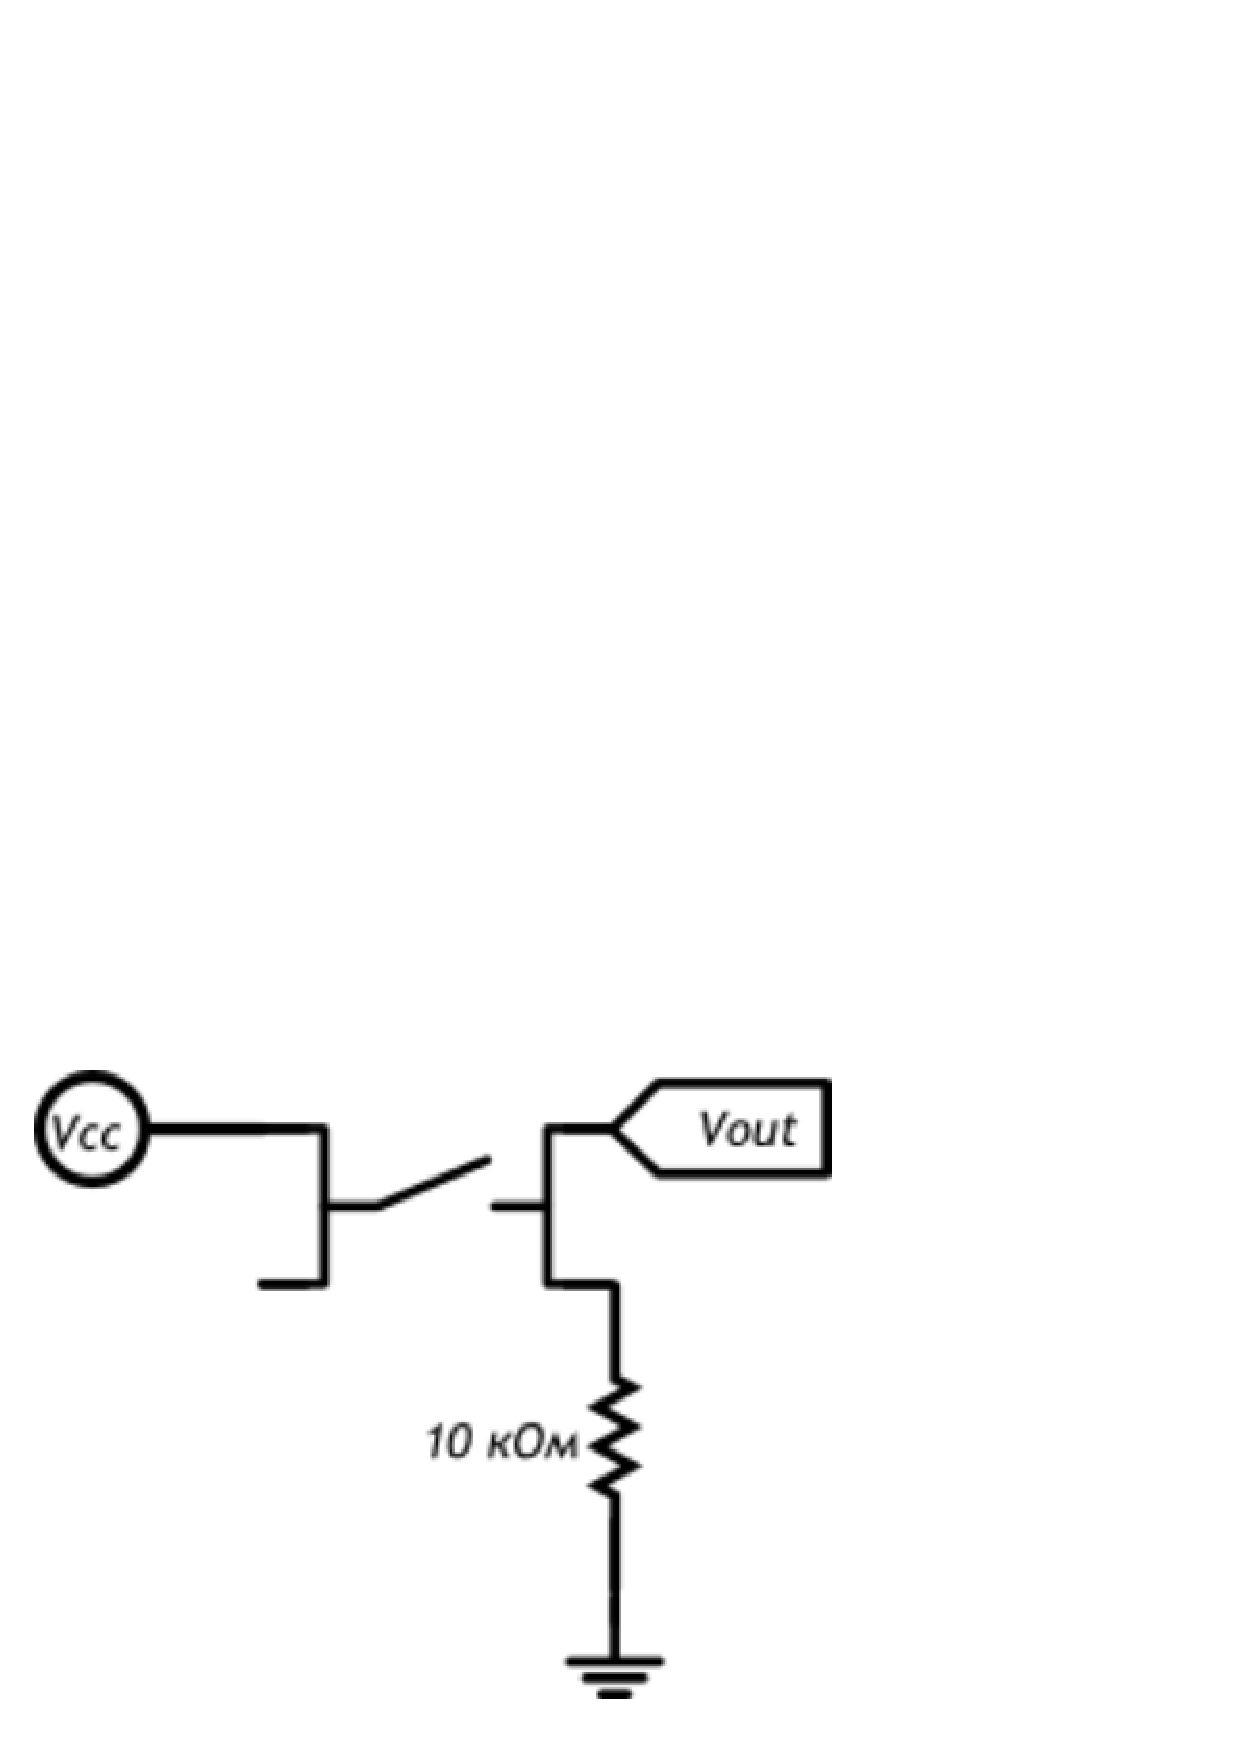
\includegraphics[height=2in]{images/ButtonShceme1.png}}
\label{ris:image}
\end{figure}

Якщо є натиснення: $V_{out} = V_{cc}$.

Якщо немає натиснення: $V_{out} = 0$.


\begin{figure}[h!]
\caption{Схема з підтягуючим резистором}
\center{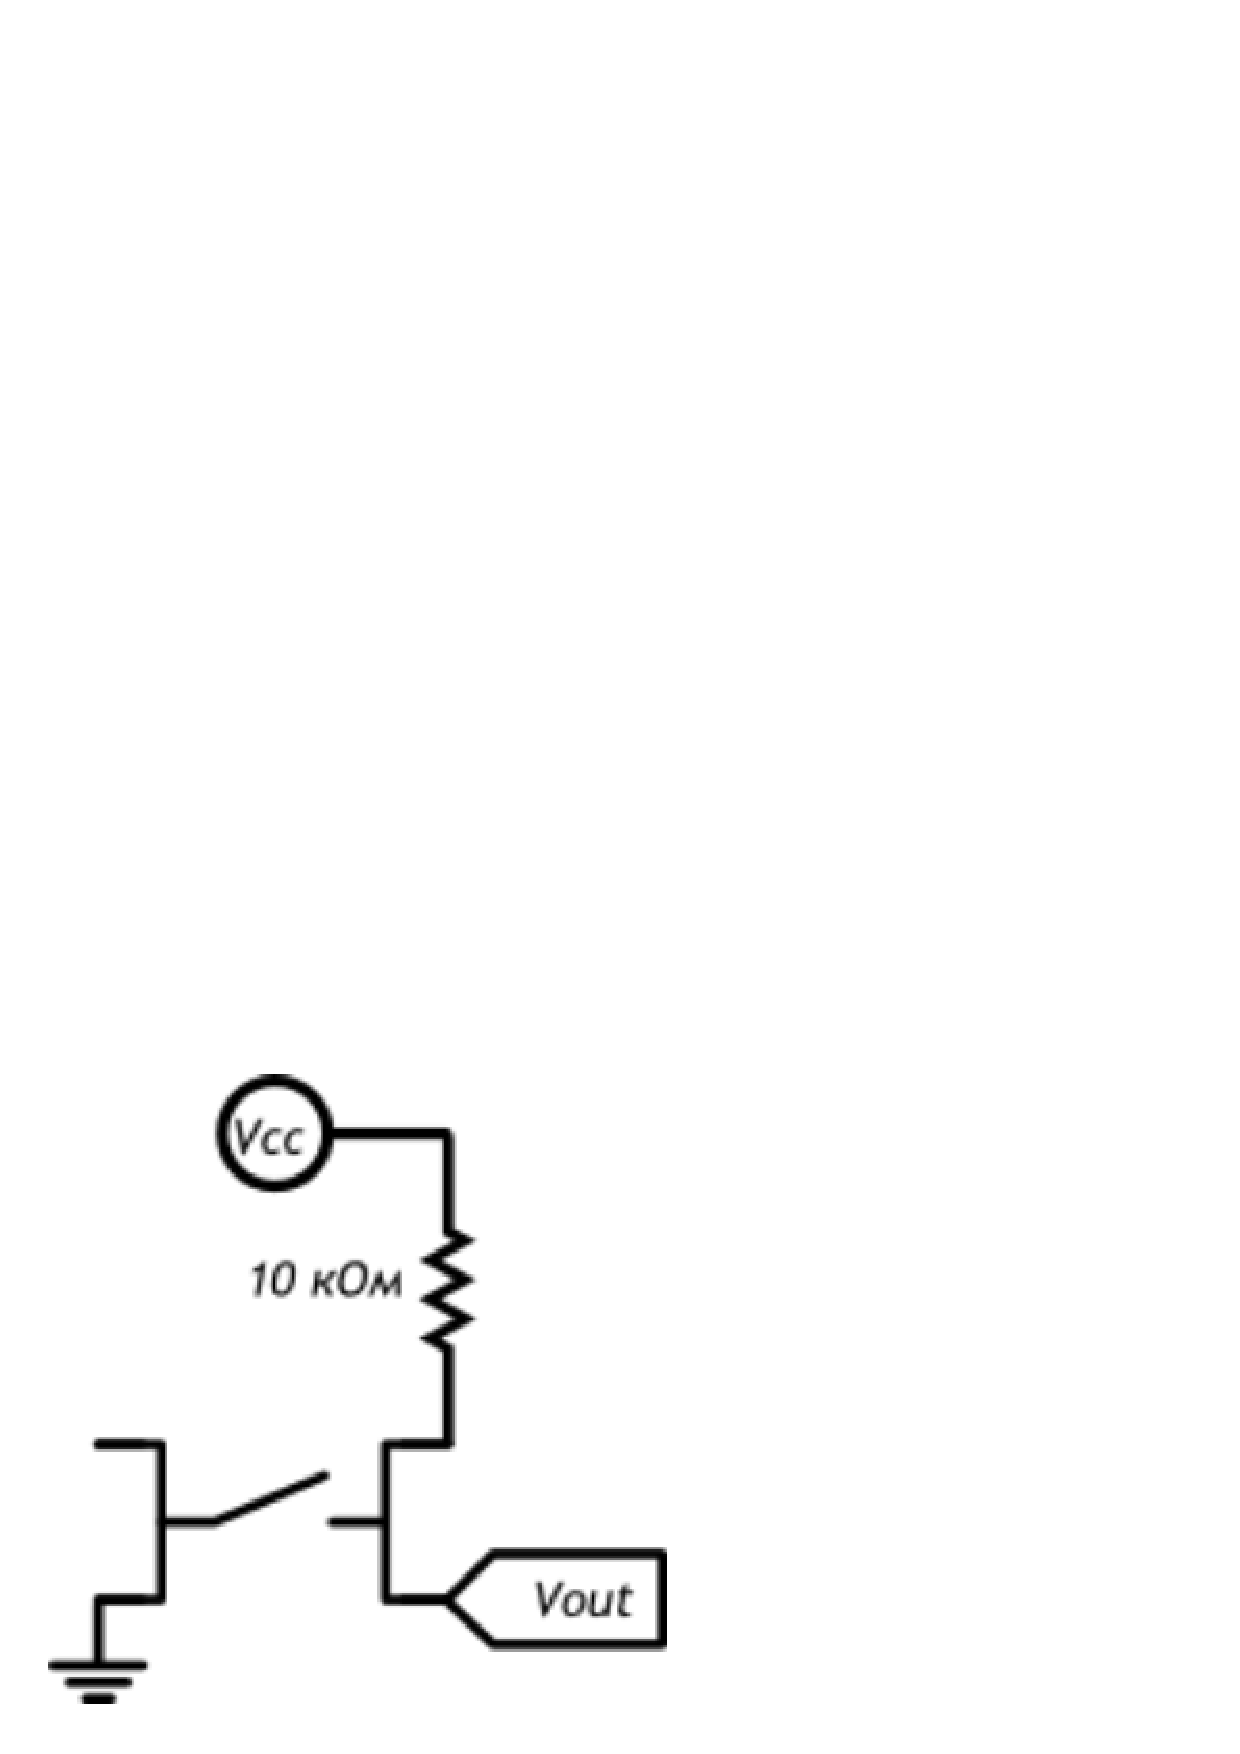
\includegraphics[height=2in]{images/ButtonShceme2.png}}
\label{ris:image}
\end{figure}

Якщо є натиснення: $V_{out} = 0$.

Якщо немає натиснення: $V_{out} = V_{cc}$.

\subsection{Широтно-імпульсна модуляція}

Мікроконтролери зазвичай не можуть видавати довіну напругу. Вони можуть видати або напругу живлення (наприклад, $5\text{В}$), або землю (тобто $5\text{В}$).

Але рівнем напруги можна управляти багатьма присторями: наприклад, яскравість світлодіода або швидкість обертання мотора. Для симуляції неповної напруги використовується ШІМ (Широтно-Імпульсна Модуляція, англ. \textit{Pulse Width Modulation} або просто \textit{PWM}).

Вихід мікроконтролера перемикається між землею і $V_{cc}$ тисячі разів в секунду. Або, як ще кажуть, має частоту в тисячі герц. Око не помічає мерехтіння більше $50 \text{Гц}$, тому нам здається, що світлодіод не мерехтить, а горить в півсили.

Аналогічно, розігнаний мотор не може зупинити вал за мілісекунди, тому ШІМ-сигнал змусить обертатися його в неповну силу.

\subsection{Дільник напруги}

Послідовно підключені резистори ділять напругу, що надходить на них у певній пропорції.

Сила струму, що протікає через резистори однакова, тому що вони з'єднані послідовно, і по закону Ома може бути розрахована як:

$$ I = \dfrac{V_{CC}}{R_1 + R_2} $$

За тим же законом Ома можна обчислити напругу $V_{out}$, яке падає на резисторі $R_2$:

$$ V_{out} = U_2 = I \cdot R_2 = \frac {R_2 \cdot V_{CC}}{R_1 + R_2} $$

З отриманої формули видно, що чим більше $R_2$ щодо $R_1$, тим більша напруга падає на ньому.

\paragraph{Зчитування резистивних сенсорів.}

Якщо замість $R_2$ використовувати не постійний резистор, а датчик, який змінює свой опір, $V_{out}$ буде залежати від вимірюваного значення.

\begin{figure}[h!]
\center{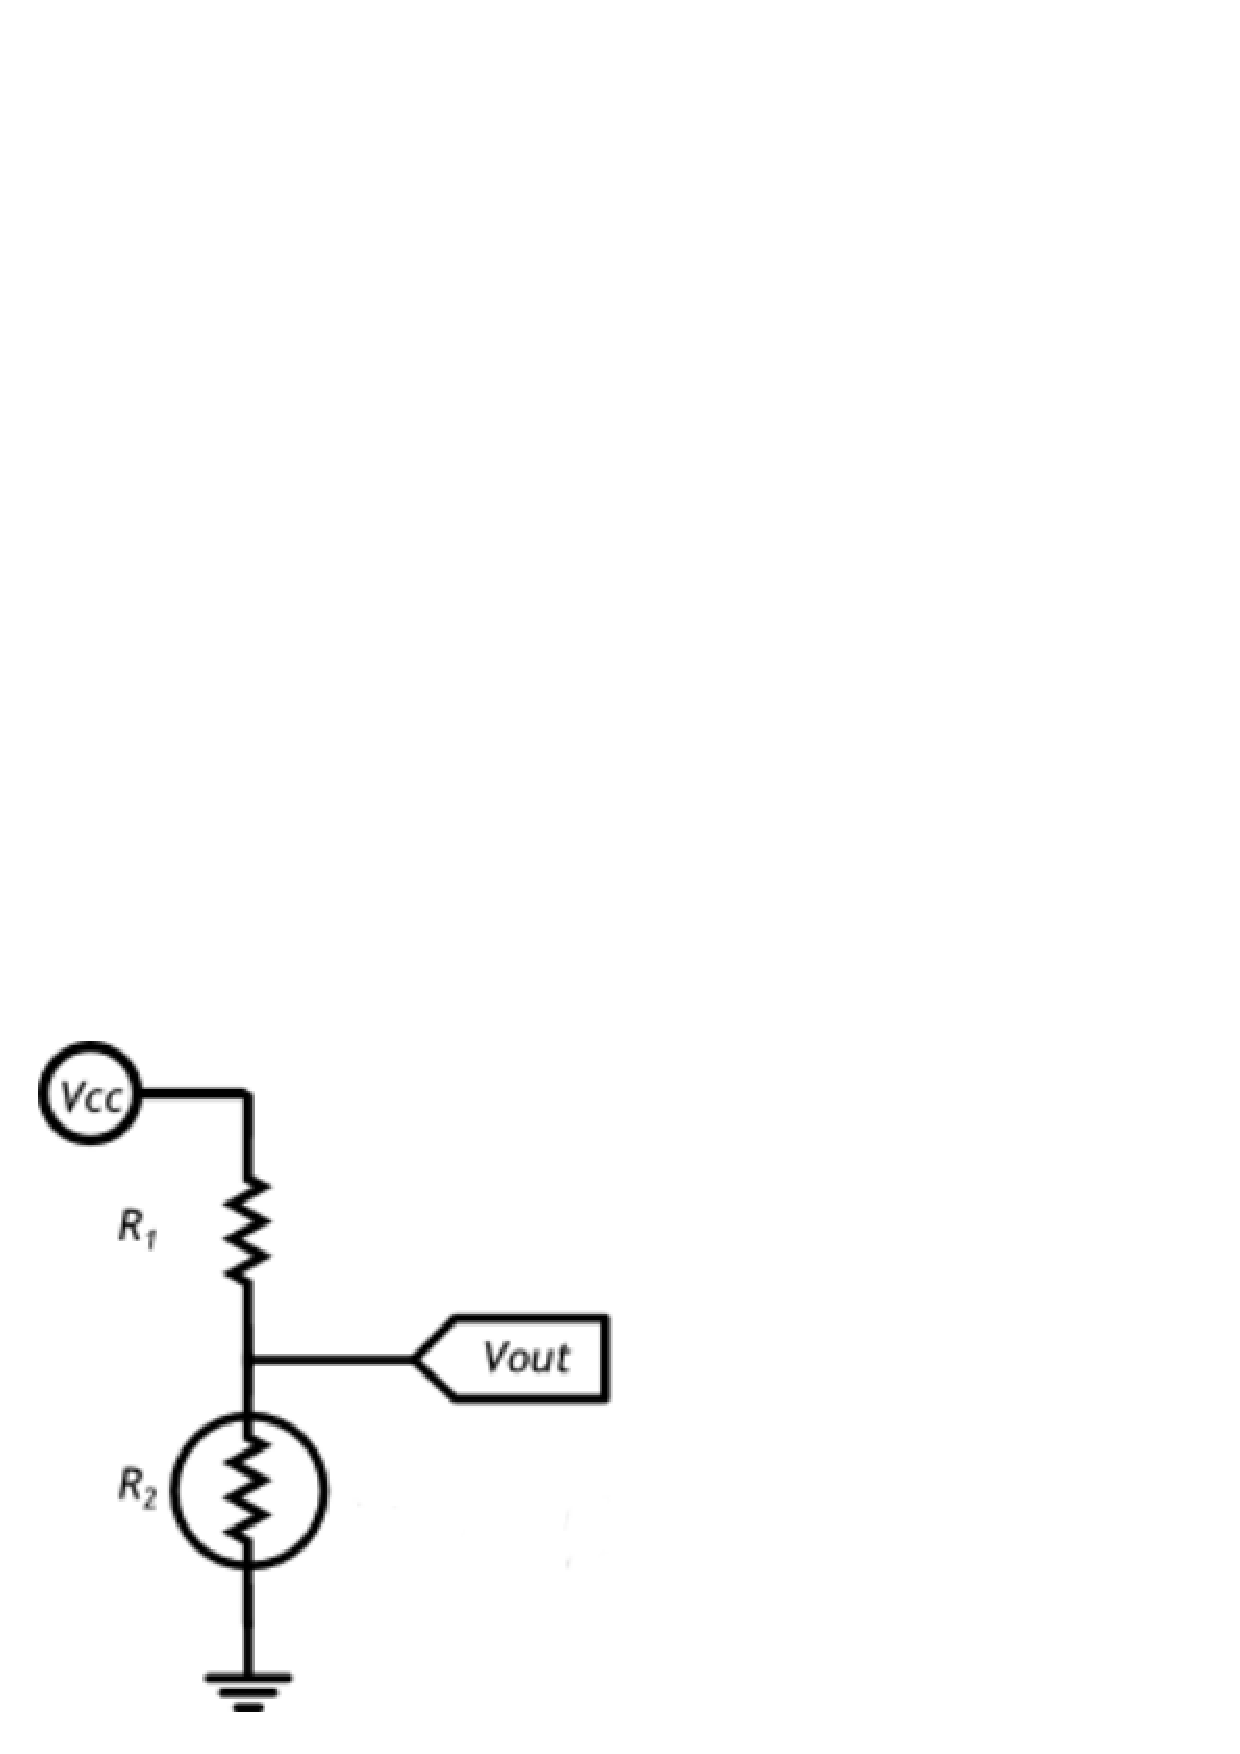
\includegraphics[height=2in]{images/VoltageDivider.png}}
\label{ris:image}
\end{figure}

Використовуючи мікроконтролер можна вимірювати напругу. Таким чином, можна використовувати властивості дільника напруги для отримання показань від сенсора.

\paragraph{Приклади резистивних датчиків}
\subparagraph{Термістор}
змінює свій опір залежно від власної температури.

\begin{figure}[h!]
\center{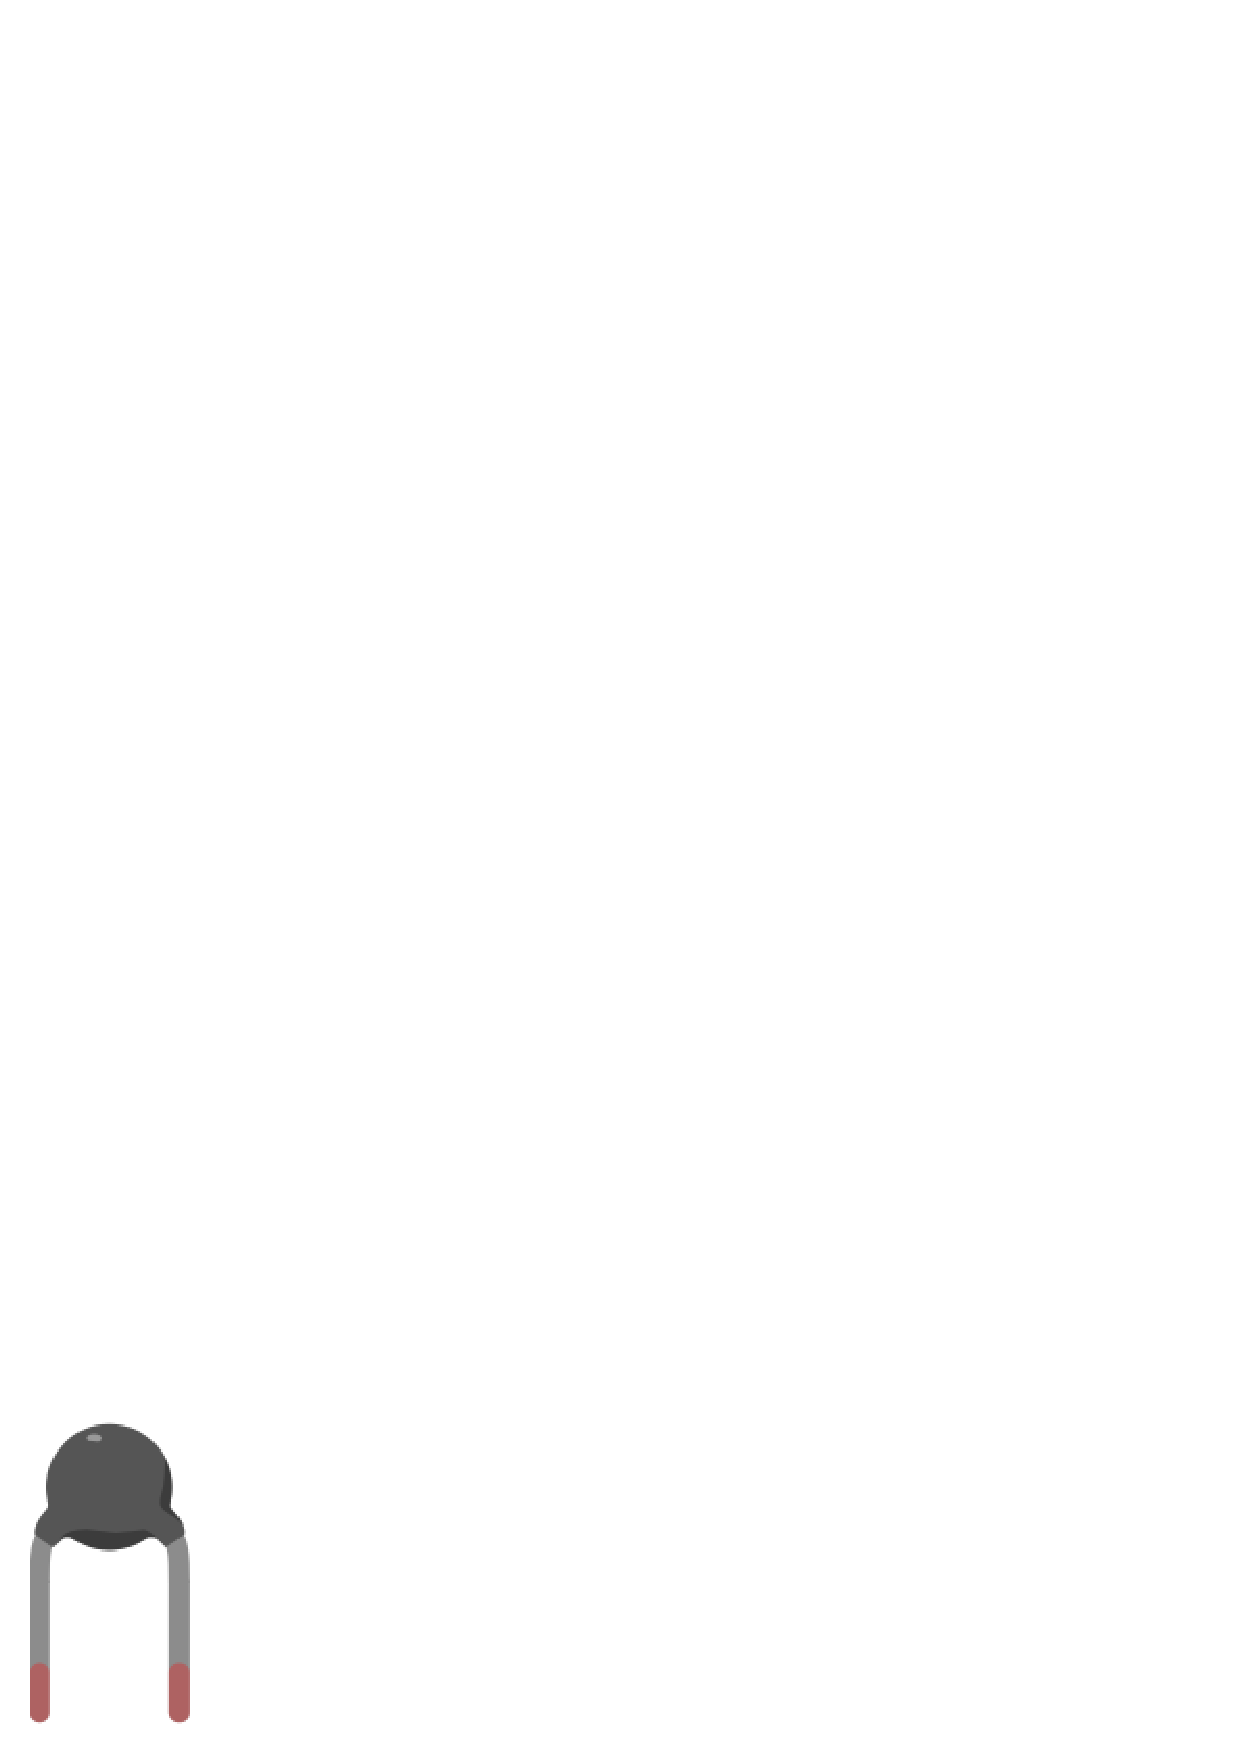
\includegraphics[height=1in]{images/Termistor.png}}
\label{ris:image}
\end{figure}

\begin{tikzpicture}[scale=2]		
	\draw[line width=2] (0,0) -- (0.3,0) -- (0.4,0.1) -- (0.5, -0.1) -- (.6, 0.1) -- (.7, -0.1) -- (.8, 0.1) -- (.9, -0.1) -- (1,0) -- (1.3, 0);
	\draw[line width=2] (0.55, -0.2) -- (0.75, 0.2) -- (1.2, 0.2);
\end{tikzpicture}

\subparagraph{Фоторезистор}
змінює свій опір залежно від сили світла, що потрапляє на його керамічну "змійку".
\begin{figure}[h!]
\center{
\includegraphics[height=0.5in]{images/Photoresistor.png}}
\label{ris:image}
\end{figure}

\begin{tikzpicture}[scale=2]		
	\draw[line width=2] (0,0) -- (0.3,0) -- (0.4,0.1) -- (0.5, -0.1) -- (.6, 0.1) -- (.7, -0.1) -- (.8, 0.1) -- (.9, -0.1) -- (1,0) -- (1.3, 0);
	\draw[line width=2] (0.65,0) circle (0.4);
	\draw[->, line width=2] (1.05, .75) -- (0.76, .41);
	\draw[->, line width=2] (1.2, .7) -- (0.9, .35);
\end{tikzpicture}

\subparagraph{Потенціометр}
ще називають змінним резистором, тримерами. Це дільник з двох резисторів в одному корпусі. Тому у нього 3 ноги: харчування, вихід, земля.
\begin{figure}[h!]
\center{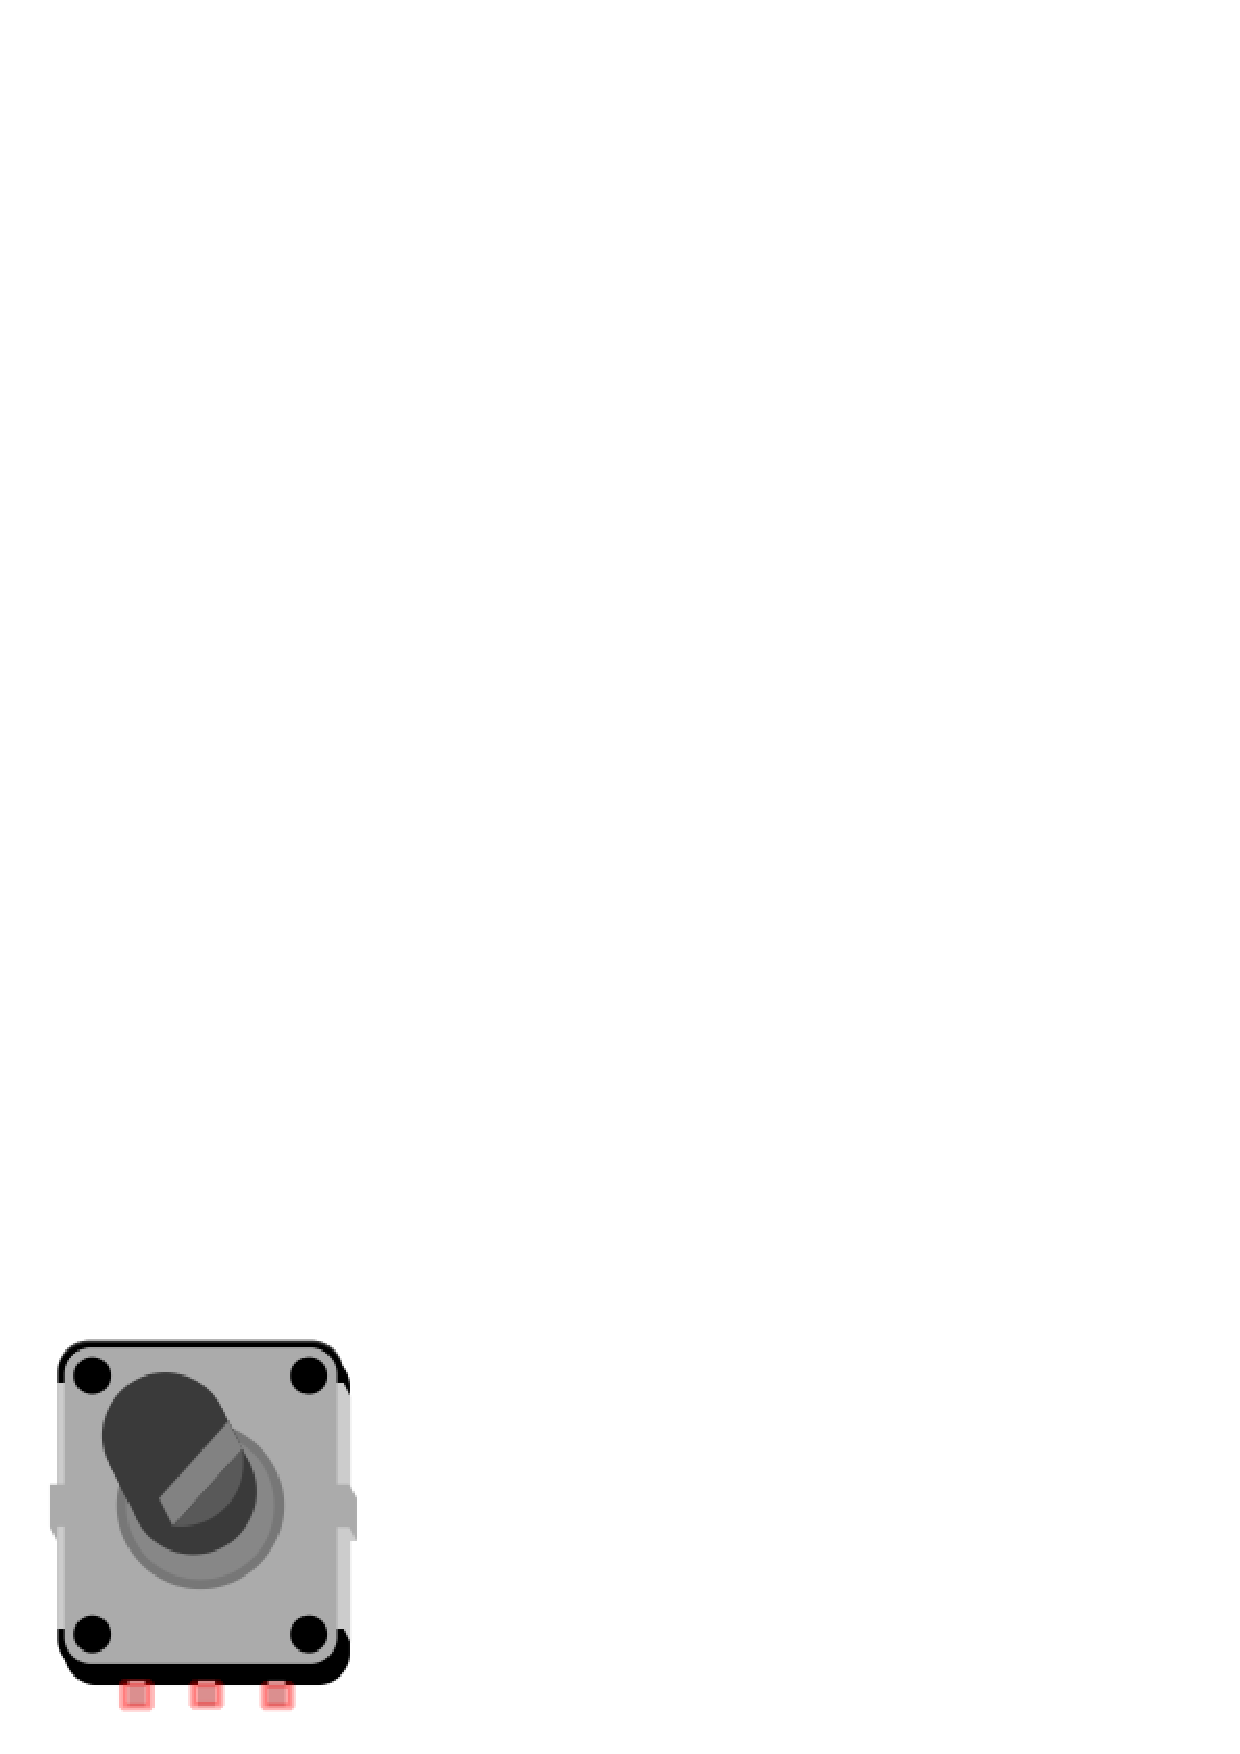
\includegraphics[height=1in]{images/POT.png}}
\label{ris:image}
\end{figure}

\begin{tikzpicture}[scale=2]		
	\draw[line width=2] (0,0) -- (0.3,0) -- (0.4,0.1) -- (0.5, -0.1) -- (.6, 0.1) -- (.7, -0.1) -- (.8, 0.1) -- (.9, -0.1) -- (1,0) -- (1.3, 0);
	\draw[line width=2] (0.75, 0.2) -- (1.2, 0.2);
	\draw[->, line width=2] (0.75, 0.2) -- (0.49, -0.3);
\end{tikzpicture}

Співвідношення $R_1$ і $R_2$ змінюється поворотом ручки. Від $100\%$ на користь $R_1$ до $100\%$ на користь $R_2$.

\subsection{Біполярний транзистор}

Транзистор~-- це електронна кнопка. На кнопку натискають пальцем, а на біполярний транзистор~-- струмом.

\begin{figure}[h!]
\center{
\includegraphics[height=1in]{images/BipolarTransistor.png}}
\label{ris:image}
\end{figure}

\begin{tikzpicture}[scale=1]		
	\draw[line width=2] (0,0) -- (1.6,0);
	\draw[line width=2] (1.6,0.7) -- (1.6,-0.7);
	\draw[line width=2] (2.5,1.5) -- (2.5,0.84) -- (1.6, 0);	
	\draw[line width=2] (2,0) circle (1);
	\draw[line width=2] (2.5,-0.84) -- (2.5,-1.5);
	\draw[->, line width=2] (1.6, 0) -- (2.5, -0.84);
	\node[below left, text=gray] at (1,0) {Б};
	\node[right, text=gray] at (2.5,1) {К};
	\node[right, text=gray] at (2.5,-1.1) {E};	
\end{tikzpicture}

Транзистори використовують для управління потужними джерелами струму за допомогою слабких сигналів з мікроконтролера.

Нога, що виконує роль «кнопки» називається база (англ. \textit{base}).
Поки через базу тече невеликий струм, транзистор відкритий:
Великий струм може втікати в колектор (англ. \textit{collector}) і витікати з емітера (англ. \textit{emitter})

\paragraph{Основні характеристики}
\begin{center}
\begin{tabular}{|l|c|c|}
\hline
\textit{Назва} & \textit{Позначення} & \textit{Одиниці виміру} \\
\hline
Максимальна напруга колектор-емітер & $V_{CE}$ & Вольт \\
\hline		
Максимальний струм через колектор & $I_C$ & Ампер \\
\hline
Коефіцієнт посилення & $h_{fe}$ & ~ \\
\hline
\end{tabular}
\end{center}

Типова схема підключення

Транзистор підсилює максимально допустимий струм в $h_{fe}$ раз:

$$ I_{CE} = I_{BE} \cdot h_{fe} $$

Приклад розрахунку

Якщо керуючий сигнал на базі транзистора з $h_{fe}$ і резистором номіналом $1 \text{кОм}$ становить $5 \text{В}$:

Який максимальний струм зможе пропустити через себе транзистор ($I_{BE}$)?

Яким за величиною буде керуючий струм ($I_{CE}$)?

$V_B = 5\text{В}$,
$R = 1\text{кОм}$,
$h_{fe} = 50$.


$ I_{BE} = \dfrac{V_B}{R} = \dfrac{5\text{В}}{1000\text{Ом}} = 5 \cdot 10^{-3} \text{А} $.

$I_{CE} = I_{BE} \cdot h_{fe} = 250 \cdot 10^{-3} \text{А}$.

Отже, якщо на базу подається $5\text{В}$ через резистор в $1\text{кОм}$, транзистор відкриється настільки, що зможе пропустити до $250\text{мА}$. При цьому керуючий струм складе всього $5\text{мА}$.

\subsection{Польовий транзистор}

Польовий MOSFET-транзистор~-- ключ для управління великими струмами за допомогою невеликого напруги.

\begin{figure}[h!]
\center{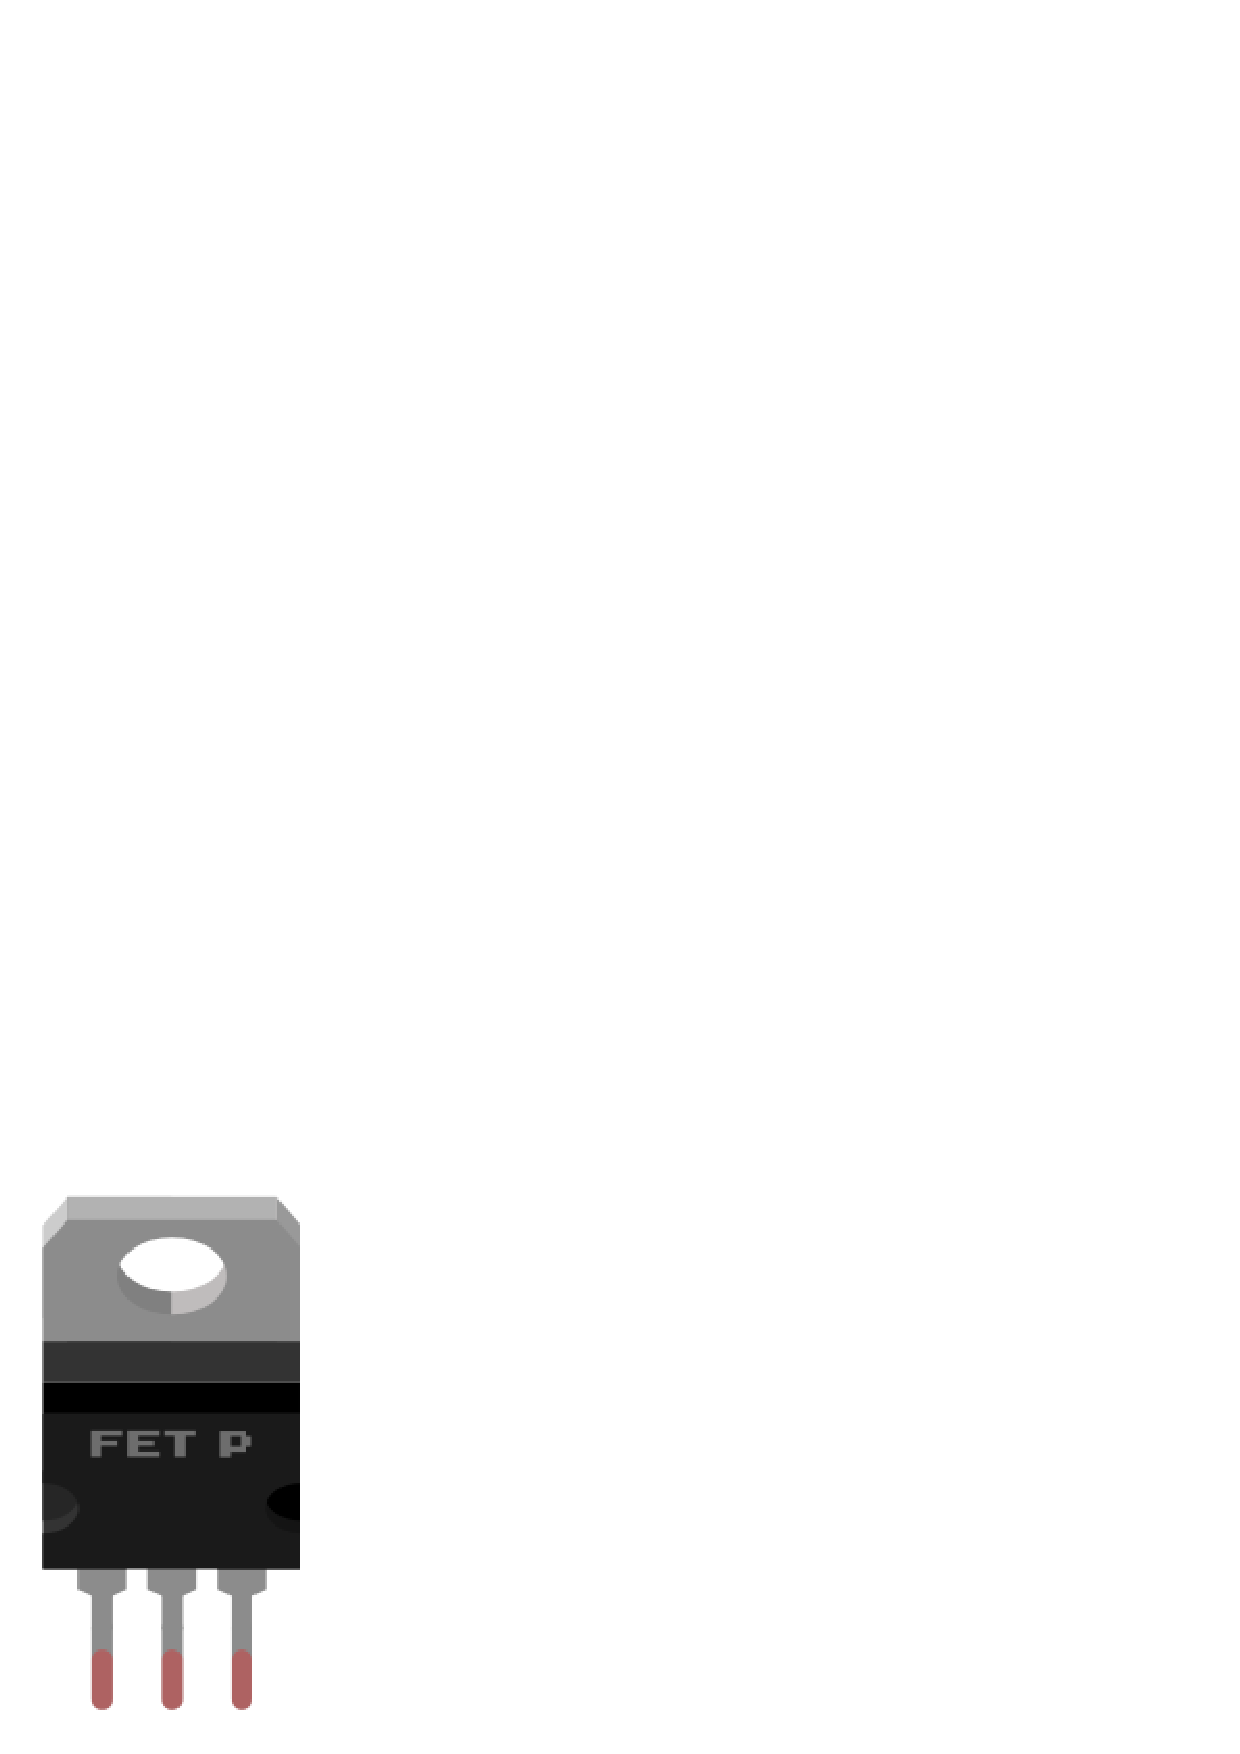
\includegraphics[height=1in]{images/PoleTransistor.png}}
\label{ris:image}
\end{figure}

\begin{tikzpicture}[scale=1]		
	\draw[line width=2] (0, -0.7) -- (1.7,-0.7) -- (1.7,0.7);
	\draw[line width=2] (2.5,1.5) -- (2.5,0.7) -- (1.9, 0.7);	
	\draw[line width=2] (2,0) circle (1);
	\draw[line width=2] (1.9, -0.7) -- (2.5,-0.7) -- (2.5, -1.5);
	\draw[->, line width=2] (2.5, 0) -- (1.9, 0);
%	\draw[densely dashed, line width=2] (1.9, 0.7) -- (1.9, -0.7);

	\draw[line width=2] (1.9, -0.7) -- (1.9,-0.4);
	\draw[line width=2] (1.9, 0.7) -- (1.9,0.4);
	\draw[line width=2] (1.9, 0.25) -- (1.9, -0.25);

	\node[below left, text=gray] at (1,0) {З};
	\node[right, text=gray] at (2.5,1) {С};
	\node[right, text=gray] at (2.5,-1.1) {В};	
\end{tikzpicture}

"Кнопка" називається затвором (англ. \textit{gate}). Поки на затворі є невелика напруга, транзистор відкритий: великий струм може втікати в стік (англ. \textit{drain}) і витікати з витоку (англ. \textit{source}).

На відміну від біполярного транзистора польовий контролюється саме напругою, а не струмом. Тобто у відкритому стані струм через затвор не проходить.

Використовуйте MOSFET для управління великими струмами, від сотень міліампер, коли біполярного транзистора вже не досить.

\paragraph{Основні характеристики}
\begin{center}
\begin{tabular}{|l|c|c|}
\hline
\textit{Назва} & \textit{Позначення} & \textit{Одиниці виміру} \\
\hline
Максимальна напруга стік-витік & $V_{DS}$ & Вольт \\
\hline		
Максимальний струм через стік & $I_D$ & Ампер \\
\hline
Опір стік-витік & $R_{DSon}$ & Ом \\
\hline
Потужність, що розсіюється & $P_D$ & Ватт \\
\hline
\end{tabular}
\end{center}

Транзистор не ідеальний і частина пропускної потужності перетворюється в тепло.

$ P_H = I^2 \cdot R_{DSon} $

Якщо $P_H$ перевищить $P_D$, без використання додаткового охолодження транзистор згорить.

\subsection{П'єзодинамік}

П'єзогенератор звуку (англ. \textit{buzzer}) переводить змінну напругу в коливання мембрани, яка в свою чергу створює звукову хвилю. П'єзодинамік~-- це конденсатор, який звучить при зарядці і розрядці.

\paragraph{Основні характеристики}
\begin{center}
\begin{tabular}{|l|c|c|}
\hline
\textit{Назва} & \textit{Позначення} & \textit{Одиниці виміру} \\
\hline
Номінальна напруга & $V$ & Вольт \\
\hline		
Гучність (на заданій відстані) & $P$ & Децибел \\
\hline
Пікова частота & $f_P$ & Герц \\
\hline
Ємність & $C$ & Фарад \\
\hline
\end{tabular}
\end{center}

\paragraph{Підключення з регулюванням гучності.} 

За допомогою потенціометра можна зменшити струм за рахунок чого зменшиться гучність.
За допомогою ризистора можна вирівняти напругу поки транзистор закритий.

\begin{figure}[h!]
\center{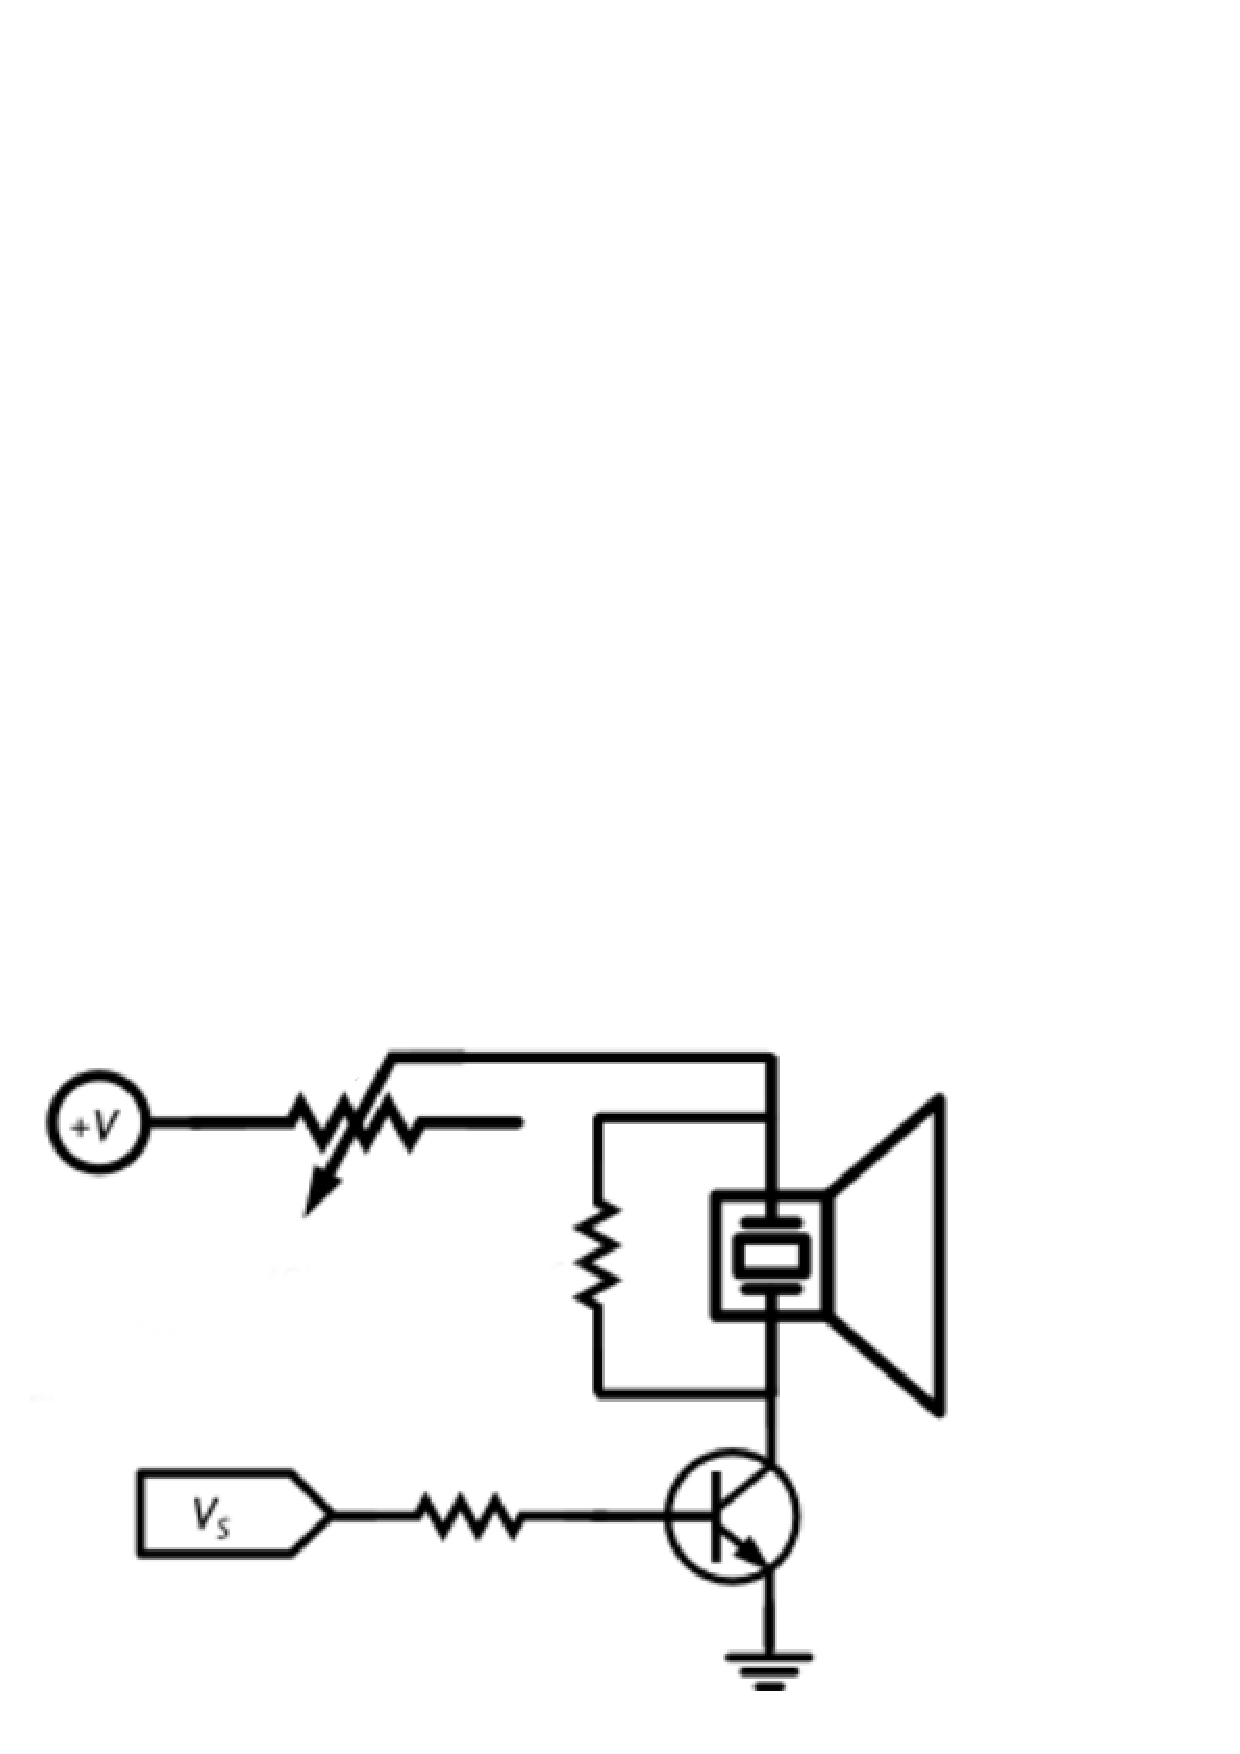
\includegraphics[height=2.5in]{images/BuzzerConnection.png}}
\label{ris:image}
\end{figure}

\subsection{Мотор}

Мотор перетвроює електричну енергію в механічну енергію обертання.

\begin{figure}[h!]
\center{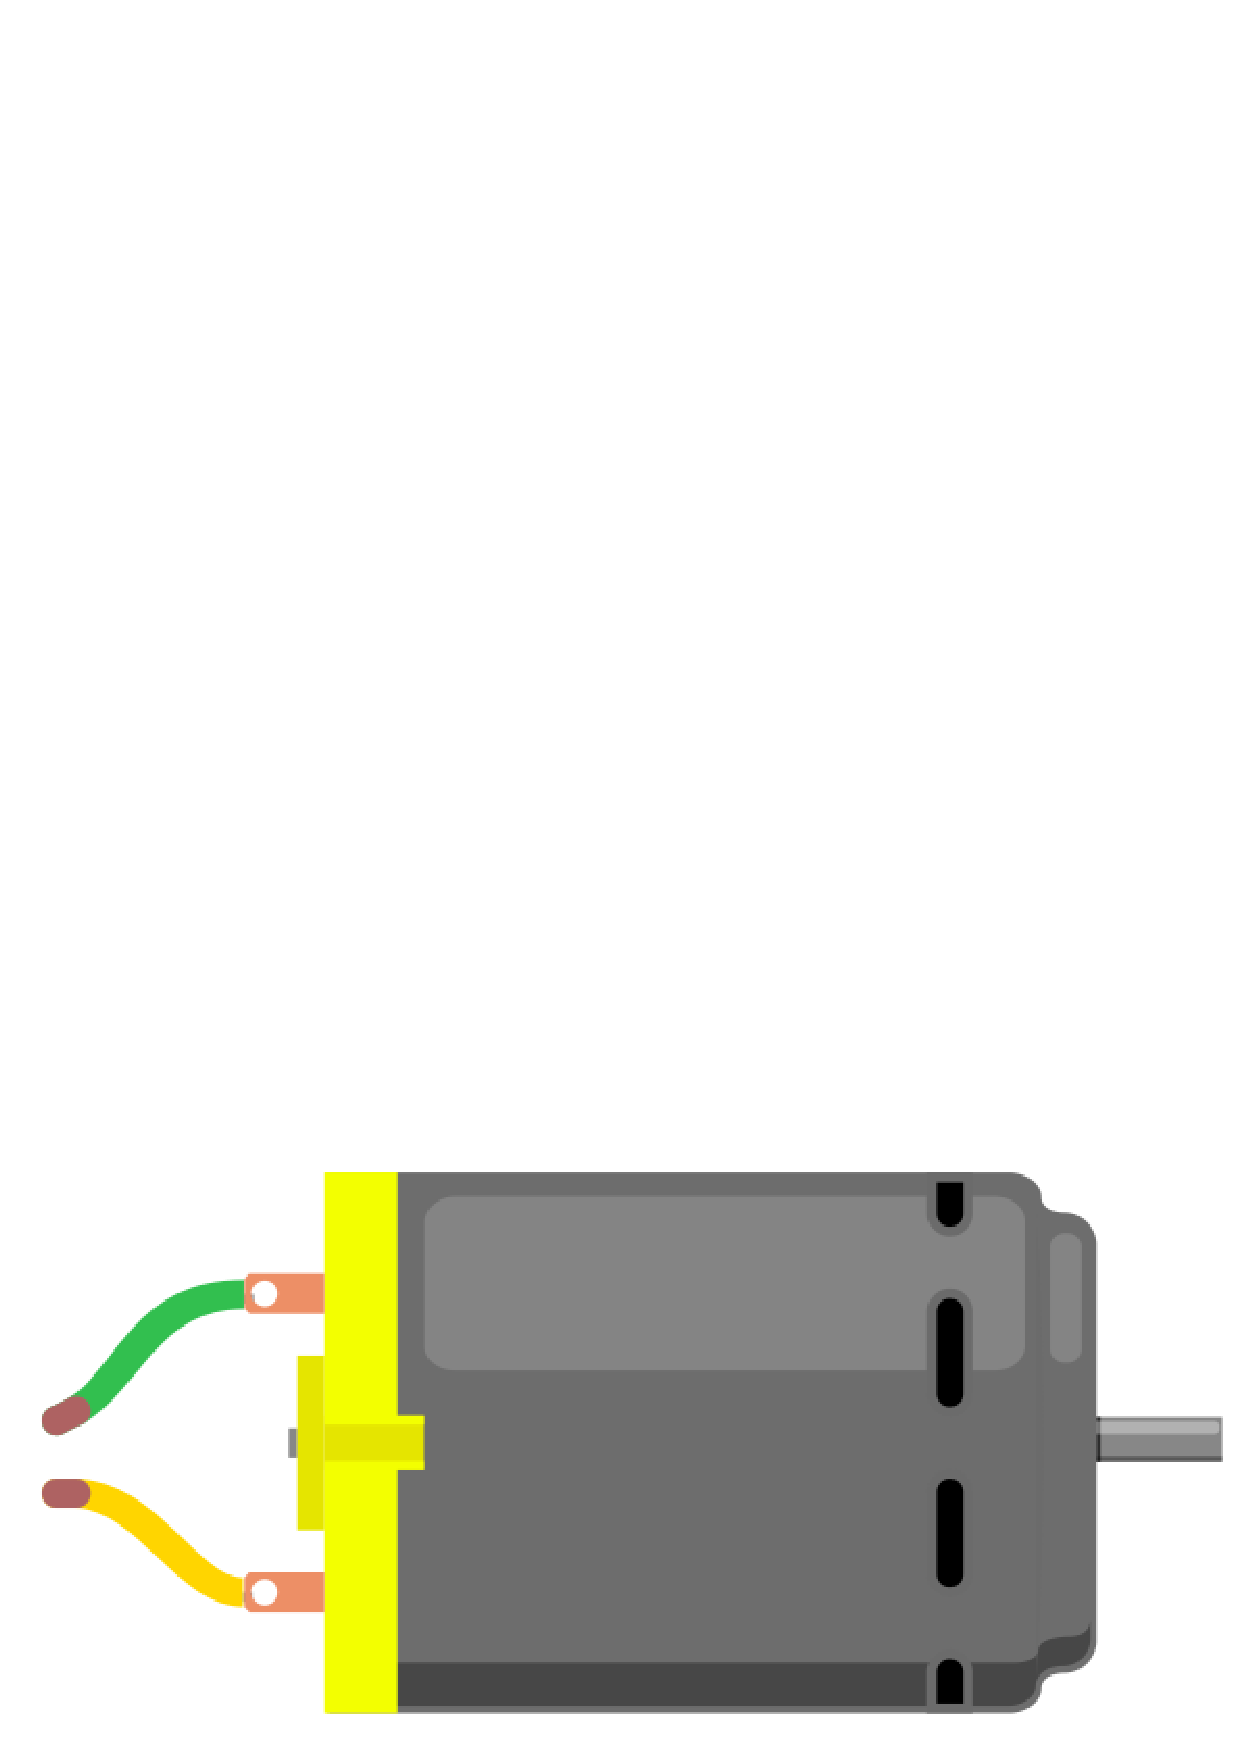
\includegraphics[height=1in]{images/Motor.png}}
\label{ris:image}
\end{figure}

\begin{tikzpicture}[scale=1]		
	\draw[line width=2] (0, 0) -- (0, 1);
	\draw[line width=2] (0, 3) -- (0, 4);
	\draw[line width=2] (0, 2) circle (1);
	\node[scale=3] at (0, 2) {M};
\end{tikzpicture}

Найпростіший вид мотора~-- колекторний. При подачі напруги в одному напрямку вал крутиться за годинниковою стрілкою, в зворотному напрямку~-- проти годинникової.

\paragraph{Основні характеристики}
\begin{center}
\begin{tabular}{|l|c|c|}
\hline
\textit{Назва} & \textit{Позначення} & \textit{Одиниці виміру} \\
\hline
Номінальна напруга & $V$ & Вольт \\
\hline		
Струм споживання без навантаження & $I_F$ & Ампер \\
\hline
Струм споживання при блокуванні & $I_S$ & Ампер \\
\hline
Швидкість обертання без навантаження & $\omega$ & $c^{-1}$ \\
\hline
Максимальний крутний мометн & $\tau$ & Н$\times$м \\
\hline
\end{tabular}
\end{center}

Мотори~-- потужні споживачі з рядом побічних ефектів. Для управління ними необхідні додаткові компоненти.

Для використання мотора доцільніше використовувати додаткове джерело живлення з рекомендованою для мотора напругою (+9V).
За допомогою транзистора можна управляти потужним моторм за допомого слабкого сигналу $V_S$.
ШІМ-сигнал використовують для регулювання швидкістю обертання вала.
Під час роботи мотор створює електромагнітні шуми. Використання конденсатора дозволяє згладити пульсації.
Коли відбувається гальмування мотора, він працює як генератор, створюючи напругу зворотної полярності. Діод потрібен для пропускання утвореного струму чез себе. Без діода вийде з ладу керуючий транзистор.

\begin{figure}[h!]
\center{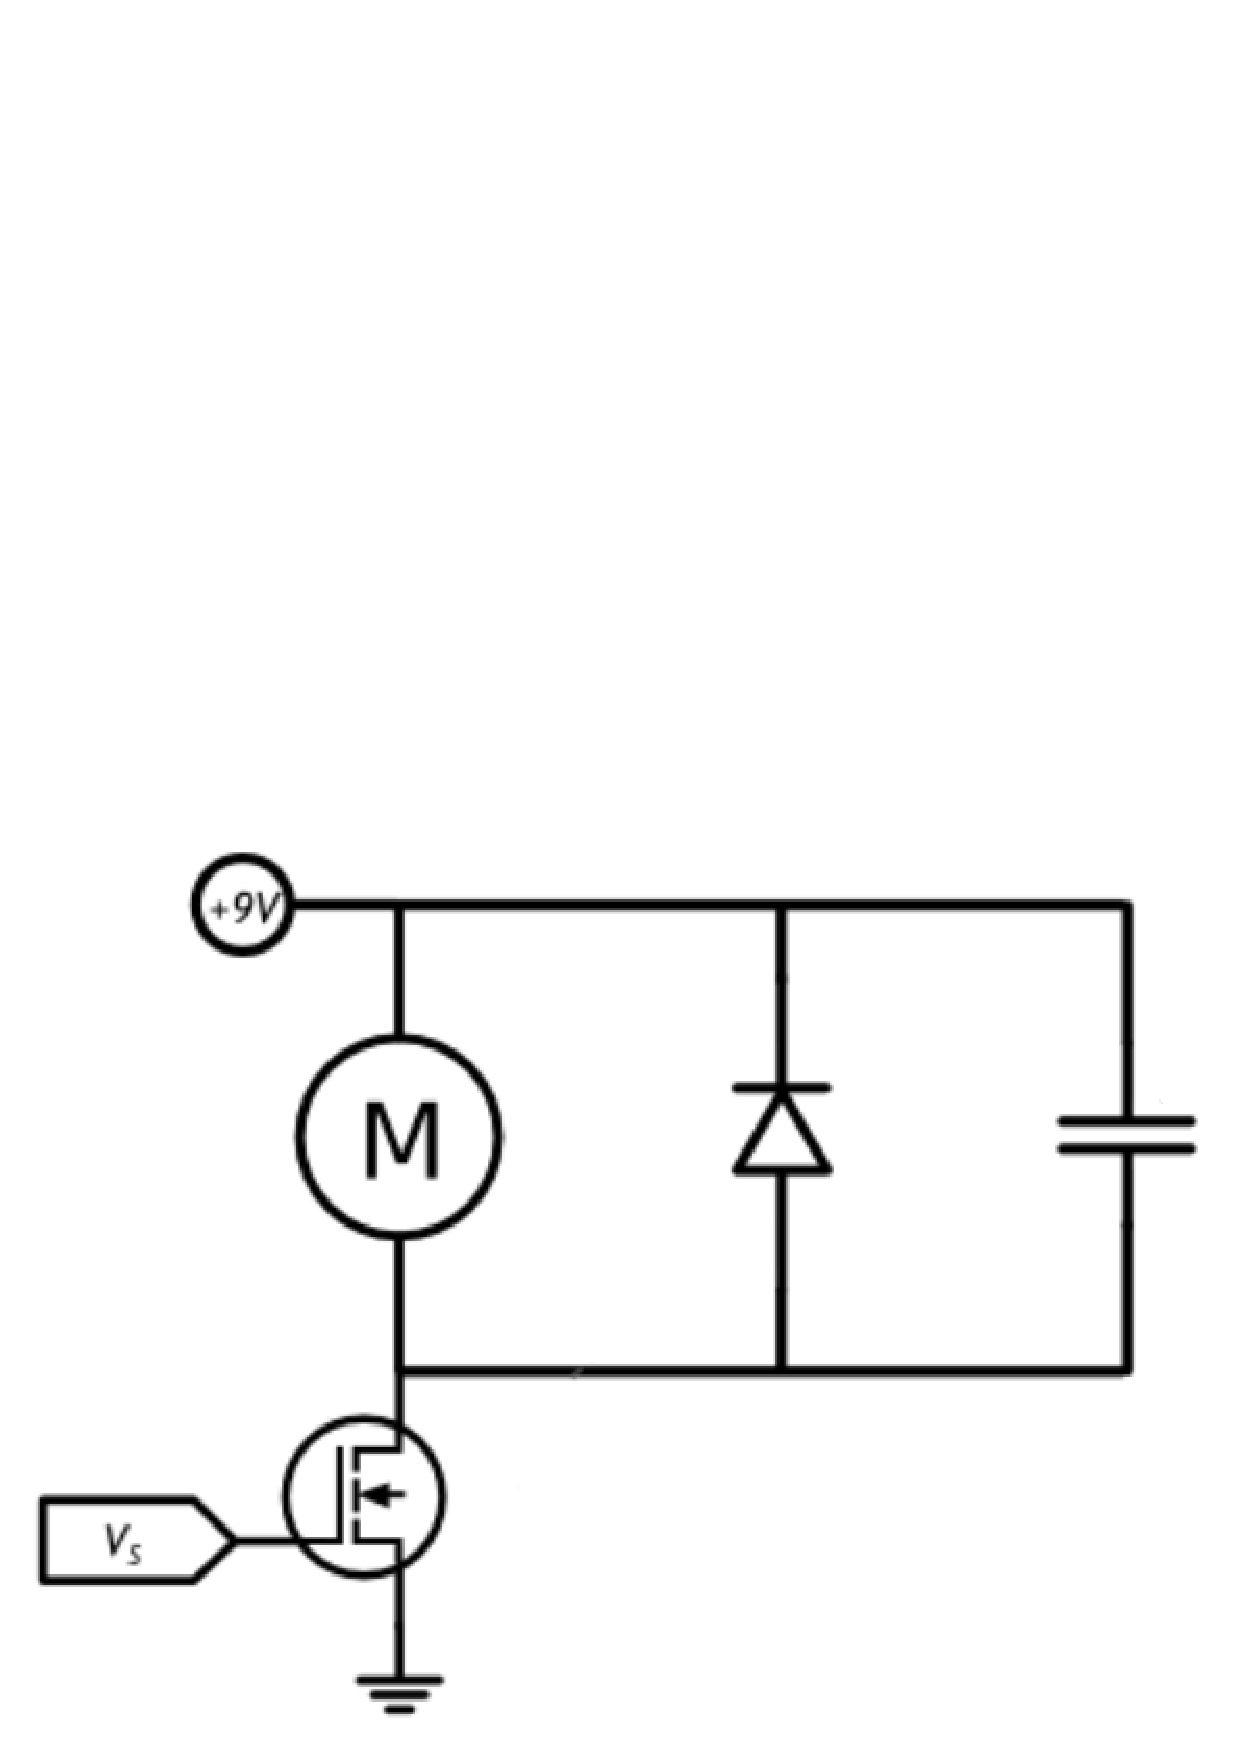
\includegraphics[height=3in]{images/MotorConnection.png}}
\label{ris:image}
\end{figure}
%=================================================

\chapter{Основи роботи з Arduino}

\section{Arduino IDE}

\section{Fritzing}

\chapter{Програмування в середовищі\\Arduino IDE}

\section{Змінні}

\subsection{Типи даних}

Комп'ютери та Arduino в тому числі, працюють з різними типами даних. В їх основі лежить арифметично-логічний пристрій (АЛП), що виконує арифметичні і логічні операції з клітинками пам'яті: $R1 + R2$, $R3 * R7$, $R4 \& R5$ і т.д. Для АЛП немає різниці, який тип даних відображати користувачеві: текст, цілі числа, числа з плаваючою комою або навіть частина програмного коду.

Команди для цих операцій надходять від компілятора, а команди компілятору передаються від користувача. Саме програміст, визначає для компілятора, що це значення~-- ціле, а інше значення - число з плаваючою комою.

\paragraph{Характеристика основних типів даних в Arduino IDE}

Оболонка для програмування Arduino по суті являє з себе мову \code{C++} з підтримкою великої кількості бібліотек для полегшення процесу написання програм. \code{C++} пропонує широкий вибір різних типів даних.

Нижче представлений список основних типів даних, які використовуються в скетчах Arduino. Поруч з кожним типом даних вказано його розмір. Зверніть увагу, сто змінні типу \code{signed} дають можливість оперувати позитивними і від'ємними числами, а змінні типу \code{unsigned} допускають тільки роботу з додатними значеннями.

    \code{boolean} (8 біт)~-- просте логічне \code{true / false}
    
    \code{byte} (8 біт)~-- \code{unsigned} число в діапазоні від $0-255$
    
    \code{char} (8 біт)~-- \code{signed} число в діапазоні від $-128$ до $127$. У деяких випадках компілятор буде інтерпретувати цей тип даних як символ, що може призвести до несподіваних результатів.
    
    \code{unsigned char} (8 біт)~-- то ж що і \code{byte}; для ясності коду рекомендується замість цього типу даних використовувати \code{byte}.
    
    \code{word} (16 біт)~-- \code{unsigned} число в діапазоні від $0$ до $65535$
    
    \code{unsigned int} (16 біт)~-- те саме, що і \code{word}. Рекомендується замінювати типом даних \code{word} для скорочення коду і ясності
    
    \code{int} (16 біт)~-- \code{signed }число в діапазоні від $-32768$ до $32767$. Один з найпоширеніших типів даних, який дуже часто використовується для оголошення змінних в скетчах-прикладах для Arduino, вбудованих в Arduino IDE
    
    \code{unsigned long} (32 біта)~-- \code{unsigned} число в діапазоні від $0-4,294,967,295$. Найчастіше цей тип даних використовується для зберігання результатів функції \code{millis()}, яка повертає кількість мілісекунд, протягом якого виконувалась дастина коду.
    
    \code{long} (32 біта)~-- \code{signed} число в діапазоні від $-2,147,483,648$ до $2,147,483,647$
    
    \code{float} (32 біта)~-- \code{signed} число в діапазоні від $-3.4028235\cdot 10^{38}$ до $3.4028235\cdot 10^{38}$. Числа з плаваючою комою не характерні для Arduino і компілятору доведеться довше опрацьовувати дані. Так що рекомендується за можливості їх уникати.


\section{Структури}

\subsection{Базовий код для програмування план Arduino}
Функція  \code{setup()} викликається на початку скетчу. Вона використовується для ініціалізації змінних, настройки режимів роботи пінів (на введення або на виведення). Функція \code{setup()} виконується один раз після подачі живлення або перезавантаження плати Arduino.

Після виконання функції \code{setup()}, циклічно виконується функція \code{loop()}, яка безпосередньо є основою програми для управління платою Arduino.

Код, наведений нижче, не виконує ніяких завдань, але його структура корисна як база для всіх програм. Крім того, зверніть увагу на те, як залишаються коментарі в скетчах.

Кожен рядок, який починається з (\code{//}) не читатися компілятором, так що у ньому можна записувати будь-які дані.


\newpage

Програмний код:

\begin{lstlisting}[label=some-code,caption=Структура програми]
int void() {
	for (int i=0; i<5; i++) {
		while (true) {
			docool();		
		}	
	}
// коментарі українською
}
\end{lstlisting}	

\subsection{Умовний оператор}

Вираз \code{if()} є основним для всіх керуючих структур в програмуванні. Цей вираз дозволяє вам здійснювати чи ні певним чином впливати залежно від умови, що є \code{true} (виконується) або \code{false} (не виконується). Синтаксис умови \code{if} виглядає наступним чином:

\begin{lstlisting}[label=conditionoperator,caption=Умовний оператор (неповна форма)]
if (someCondition) {
	// дії, які потрібно виконати, якщо умова виконується
}
\end{lstlisting}

Так само є подібні варіації структури з використанням if-else. Виглядає це наступним чином:

\begin{lstlisting}[label=conditionoperator,caption=Умовний оператор (повна форма)]
if (someCondition) {
	// дії, які потрібно виконати, якщо умова виконується
}
else {
	// дії, які потрібно виконати, якщо умова не виконується
}
\end{lstlisting}

Також є структура else-if, за допомогою якої ви можете перевірити друга умова, якщо перше не виконується:

\begin{lstlisting}[label=conditionoperator,caption=Умовний оператор (декільки умов)]
if (someCondition) {
	// дії, які потрібно виконати, якщо умова виконується
} 
else if (anotherCondition) {
	// дії, які потрібно виконати тільки якщо не виконується перша умова
	// а друга умова виконується
}
\end{lstlisting}

Кількість розгалужень може бути необмеженою.

\subsection{Оператор вибору}

\code{switch}

\subsection{Циклічні оператори}
Циклічні оператори використовуються для повтоерння однакових або однотипних дій.

\paragraph{for}

Доцільно використовувати коли відома кількість поврень, які потрібно виконати.

\begin{lstlisting}[label=conditionoperator,caption=Оператор повторення for]
for(int i=0; i<10; i++) {
	// всі оператори всередині фігурних дужок називаються тілом циклу
	Serial.println(i);
}
\end{lstlisting}

Перший аргумент~-- початкове значення лічильника. В даному випадку стоврюється внутрішня змінна \code{i}, якій надається початкового значення 0.

Другий аргумент~-- умова за якої тіло циклу виконується. Зазвичайумова вказується як заежність від лічильника. У прикладі тіло циклу виконуватиметься поки значення лічильника буде меншим за 10.

Третій аргумент~-- спосіб зміни лічильника. У прикладі лічильник з кожною ітерацією збільшується на 1. Таким чином, враховуючи умову, тіло циклу викорається 10 разів.

Кожен аргумент не є обов'язковим і може бути пропущений під час оголошення циклу. Але для коректної роботи потрібно конторювати всі складові окремо. Навдемо приклад тієї ж програми з порожніми агрументами.

\begin{lstlisting}[label=conditionoperator,caption=Оператор повторення for]
int i = 0; // оголошення та ініціалізація лічильника за межами циклу
for(;;) {
	Serial.println(i);
	i++; // зміна значення лічильника
	if (i >= 10) break;
}
\end{lstlisting}

Для аналогічної роботи такої циклічної структури використовується оператор \code{break}, який потрібен для дострокового переривання виконання циклу.

\paragraph{Цикл while}
\paragraph{Цикл do...while}

\subsection{Масиви}

Масив~-- це набір однотипних змінних, доступ до яких здійснюється через їх індекс. У мові програмування C, на якому заснований Arduino, масиви можуть бути досить складними.

\paragraph{Створення (оголошення) масиву.} 
Всі методики, представлені нижче, підходять для створення (оголошення) масиву.

\begin{lstlisting}[label=conditionoperator,caption=Оголошення масиву]
int myInts [6];
int myPins [] = {2, 4, 8, 3, 6};
int mySensVals [6] = {2, 4, -8, 3, 2};
char message [6] = "hello";
\end{lstlisting}

Ви можете оголосити масив без його ініціалізації як \code{myInts}.

У \code{myPins} оголошується масив без безпосередньої вказівки розміру. Компілятор вважає кількість елементів і створює масив відповідного розміру.

Можна одночасно форматувати і вказати розмір вашого масиву, як, наприклад, це зроблено в \code{mySensVals}. Зверніть увагу, що при оголошенні масиву типу \code{char}, необхідний ще один елемент для зберігання обов'язкового \code{null}-символу.

\paragraph{Доступ до елементів масиву.}
Індексація в масивах починається з нуля. Тобто, перший елемент масиву буде мати порядковий номер \code{0}. Таким чином:

\code{mySensVals [0] == 2, mySensVals [1] == 4}, і так далі

Тобто, наприклад, в масиві з десяти елементів, останній елемент буде мати індекс дев'ять. наприклад:

\code{int myArray [10] = {9,3,2,4,3,2,7,8,9,11};} 
\code{myArray[9]} містить 11, а вираз \code{myArray[10]} некоректний і містить випадкові дані (іншу адресу пам'яті).

З цієї причини треба бути акуратним при доступі до масивів. Звертаючись до елементу масиву, значення якого більше ніж оголошений розмір ви счітвиете з пам'яті значення, яке призначене для інших завдань. Зчитування таких даних просто призведе до некоректних результатів роботи програми в подальшому. Також не дуже хорошою ідеєю є запис даних в довільні місця. Крім того, відстежити цю помилку при перевірці коду теж складно.

На відміну від BASIC або JAVA, компілятор C не перевіряє, чи отримуємо ми доступ до елементу масиву в попередньо оголошених межах.

Для надання значення елементу масива під номером \code{0}:

\code{mySensVals [0] = 10;}

Для отримання значення елемента масиву за номером \code{4}:

\code{x = mySensVals [4];}

\section{Функції}

\subsection{Цифрове введення/виведення}

\paragraph{digitalRead()}

\subparagraph{Опис:}

Reads the value from a specified digital pin, either HIGH or LOW.
\subparagraph{Синтакс}

\code{digitalRead(pin)}
\subparagraph{Параметри}

pin: the number of the digital pin you want to read
Returns

HIGH or LOW
Example Code

Sets pin 13 to the same value as pin 7, declared as an input.
\begin{lstlisting}[label=conditionoperator,caption=Використання функції digitalRead()]
int ledPin = 13;   // Світлодіод приєднано до піна 13
int inPin = 7;     // Кнопка приєнана до цифорового піна 7
int val = 0;       // Змінна для збереження отриманого значення

void setup()
{
  pinMode(ledPin, OUTPUT);      // Встановлення 13 піна для виведення
  pinMode(inPin, INPUT);        // Встановлення 7 піна для введення
}

void loop()
{
  val = digitalRead(inPin);     // зчитуємо значення на 7 піні
  digitalWrite(ledPin, val);    // встановлюємо значення для світлодіода рівним прочитаному занченню
}
\end{lstlisting}

Notes and Warnings

If the pin isn’t connected to anything, digitalRead() can return either HIGH or LOW (and this can change randomly).

The analog input pins can be used as digital pins, referred to as A0, A1, etc.

\paragraph{digitalWrite()}


Description

Write a HIGH or a LOW value to a digital pin.

If the pin has been configured as an OUTPUT with pinMode(), its voltage will be set to the corresponding value: 5V (or 3.3V on 3.3V boards) for HIGH, 0V (ground) for LOW.

If the pin is configured as an INPUT, digitalWrite() will enable (HIGH) or disable (LOW) the internal pullup on the input pin. It is recommended to set the pinMode() to
\code{INPUTPULLUP} % must be INPUT_PULLUP
to enable the internal pull-up resistor. See the digital pins tutorial for more information.

If you do not set the pinMode() to OUTPUT, and connect an LED to a pin, when calling digitalWrite(HIGH), the LED may appear dim. Without explicitly setting pinMode(), digitalWrite() will have enabled the internal pull-up resistor, which acts like a large current-limiting resistor.
Syntax

digitalWrite(pin, value)
Parameters

pin: the pin number

value: HIGH or LOW
Returns

Nothing
Example Code

The code makes the digital pin 13 an OUTPUT and toggles it by alternating between HIGH and LOW at one second pace.

void setup()
{
  pinMode(13, OUTPUT);          // sets the digital pin 13 as output
}

void loop()
{
  digitalWrite(13, HIGH);       // sets the digital pin 13 on
  delay(1000);                  // waits for a second
  digitalWrite(13, LOW);        // sets the digital pin 13 off
  delay(1000);                  // waits for a second
}

Notes and Warnings

The analog input pins can be used as digital pins, referred to as A0, A1, etc.


\subsection{Аналогове введення/виведення}
\subsection{Додаткове введення/виведення}
\subsection{Робота з часом}
\subsection{Математичні функції}
\subsection{Символьні функції}
\subsection{Псевдовипадкові числа}
\subsection{Бітові функції}
\subsection{Функції комунікації}


\end{document}


